% =====================================================================
%  PAPER V -- Keep Flying Whatever the Model Says:
%  Predictive Safety Filtering for Language-Model UAV Agents under
%  Adaptive Attack.            RobustUAVs.ai programme, Paper V.
%
%  Target venue: IEEE SaTML (IEEEtran conference class, double-blind).
%  NOTE ON VENUE: the SaTML 2027 paper deadline (29 Sep 2026, per a
%  secondary aggregator; confirm on satml.org) has PASSED as of this
%  draft (15 Oct 2026). Target the next SaTML cycle, or USENIX Security
%  as the fallback. Re-check page limits, artifact and ethics rules on
%  the official call before submission.
%
%  Build (standalone; the figure data are embedded below with
%  filecontents* and written next to this file on the first run):
%    pdflatex PaperV_main && bibtex PaperV_main && pdflatex PaperV_main && pdflatex PaperV_main
%
%  Every number in this file is copied from the simulation pilot's
%  results_summary.md / figdata/*.dat (non-LLM planners). Real-LLM
%  results do not exist yet; their slots are marked with \pending.
%  NEVER replace a \pending marker with a number that was not measured.
%
%  Naming note: the pilot code (attacks.py, adaptive.py) calls the
%  action-space oracle "A7" (task-brief naming). This manuscript follows
%  the research plan's ladder: A6 = action-space oracle, A7 = A6/A3
%  composed with Paper IV's covert sensing attacker.
% =====================================================================
% ---- Figure data: verbatim copies of paperV/figdata/*.dat (pilot) ----
\begin{filecontents*}[overwrite]{pv-violation_onoff.dat}
label N on on_lo on_hi off off_lo off_hi svr_on svr_on_cp95 svr_off eps_on eps_off
benign-N4 4 0 0 0.0876216 0 0 0.0876216 0 2.13979e-05 0 40 40
random-N4 4 0 0 0.0876216 0.975 0.871186 0.995573 0 2.13979e-05 0.0160357 40 40
stall-N4 4 0 0 0.0876216 0 0 0.0876216 0 2.13979e-05 0 40 40
oracle_violation-N4 4 0 0 0.0876216 1 0.912378 1 0 2.13979e-05 0.960157 40 40
oracle_denial-N4 4 0 0 0.0876216 1 0.912378 1 0 2.13979e-05 0.960086 40 40
benign-N12 12 0 1.38778e-17 0.215311 0 1.38778e-17 0.215311 0 2.03789e-05 0 14 14
random-N12 12 0 1.38778e-17 0.215311 1 0.784689 1 0 2.03789e-05 0.017102 14 14
stall-N12 12 0 1.38778e-17 0.215311 0 1.38778e-17 0.215311 0 2.03789e-05 0 14 14
oracle_violation-N12 12 0 1.38778e-17 0.215311 1 0.784689 1 0 2.03789e-05 0.960061 14 14
oracle_denial-N12 12 0 1.38778e-17 0.215311 1 0.784689 1 0 2.03789e-05 0.960041 14 14
\end{filecontents*}
\begin{filecontents*}[overwrite]{pv-admissible_shrinkage.dat}
btot area_frac sep_required_m
0 0.922364 16.0537
0.25 0.918901 16.5537
0.5 0.915443 17.0537
0.75 0.91199 17.5537
1 0.90854 18.0537
1.25 0.905095 18.5537
1.5 0.901655 19.0537
1.75 0.898218 19.5537
2 0.894786 20.0537
2.25 0.891358 20.5537
2.5 0.887934 21.0537
2.75 0.884515 21.5537
3 0.8811 22.0537
3.25 0.877689 22.5537
3.5 0.874283 23.0537
3.75 0.87088 23.5537
4 0.867483 24.0537
4.25 0.864089 24.5537
4.5 0.8607 25.0537
4.75 0.857315 25.5537
5 0.853934 26.0537
5.25 0.850557 26.5537
5.5 0.847185 27.0537
5.75 0.843817 27.5537
6 0.840454 28.0537
6.25 0.837094 28.5537
6.5 0.833739 29.0537
6.75 0.830389 29.5537
7 0.827042 30.0537
7.25 0.8237 30.5537
7.5 0.820362 31.0537
7.75 0.817028 31.5537
8 0.813699 32.0537
8.25 0.810374 32.5537
8.5 0.807053 33.0537
8.75 0.803737 33.5537
9 0.800425 34.0537
9.25 0.797117 34.5537
9.5 0.793813 35.0537
9.75 0.790514 35.5537
10 0.787219 36.0537
10.25 0.783928 36.5537
10.5 0.780642 37.0537
10.75 0.77736 37.5537
11 0.774082 38.0537
11.25 0.770808 38.5537
11.5 0.767539 39.0537
11.75 0.764274 39.5537
12 0.761014 40.0537
12.25 0.757757 40.5537
12.5 0.754505 41.0537
12.75 0.751257 41.5537
13 0.748014 42.0537
13.25 0.744774 42.5537
13.5 0.741539 43.0537
13.75 0.738309 43.5537
14 0.735082 44.0537
14.25 0.73186 44.5537
14.5 0.728643 45.0537
14.75 0.725429 45.5537
15 0.72222 46.0537
15.25 0.719015 46.5537
15.5 0.715814 47.0537
15.75 0.712618 47.5537
16 0.709426 48.0537
16.25 0.706238 48.5537
16.5 0.703054 49.0537
16.75 0.699875 49.5537
17 0.6967 50.0537
17.25 0.69353 50.5537
17.5 0.690363 51.0537
17.75 0.687201 51.5537
18 0.684043 52.0537
18.25 0.68089 52.5537
18.5 0.677741 53.0537
18.75 0.674596 53.5537
19 0.671455 54.0537
19.25 0.668319 54.5537
19.5 0.665187 55.0537
19.75 0.662059 55.5537
20 0.658936 56.0537
\end{filecontents*}
\begin{filecontents*}[overwrite]{pv-denial_vs_btot_N4_benign.dat}
btot denial lo hi denial_filter denial_envelope fr fr_lo fr_hi ir mcr area_frac eps
0 0 0 0.193608 0 0 0 0 0 0.0872321 1 0.922364 16
0.5 0 0 0.193608 0 0 0 0 0 0.110357 1 0.915443 16
1 0 0 0.193608 0 0 0 0 0 0.113571 1 0.90854 16
2 0 0 0.193608 0 0 0 0 0 0.126071 1 0.894786 16
4.371 0 0 0.193608 0 0 0 0 0 0.1925 1 0.862448 16
7.01888 0 0 0.193608 0 0 0 0 0 0.259821 1 0.826789 16
12.7178 1 0.806392 1 0.8125 0 1 1 1 1 0 0.751675 16
\end{filecontents*}
\begin{filecontents*}[overwrite]{pv-denial_vs_btot_N12_benign.dat}
btot denial lo hi denial_filter denial_envelope fr fr_lo fr_hi ir mcr area_frac eps
0 0 0 0.434482 0 0 0 0 0 0.0659048 1 0.961215 5
0.5 0 0 0.434482 0 0 0 0 0 0.104381 1 0.957743 5
1 0 0 0.434482 0 0 0 0 0 0.0973333 1 0.954278 5
2 0 0 0.434482 0 0 0.00342857 0.00114286 0.00571429 0.126095 1 0.947366 5
4.371 0 0 0.434482 0 0 0.00457143 0.00114286 0.008 0.153524 1 0.931075 5
7.01888 0 0 0.434482 0 0 0 0 0 0.263238 1 0.913045 5
12.7178 1 0.565518 1 0 0 1 1 1 1 0 0.874827 5
\end{filecontents*}
\begin{filecontents*}[overwrite]{pv-denial_vs_btot_N4_oracle_denial.dat}
btot denial lo hi denial_filter denial_envelope fr fr_lo fr_hi ir mcr area_frac eps
0 1 0.806392 1 0.1875 0.8125 0.00357143 0.00178571 0.00571429 1 0 0.922364 16
0.5 1 0.806392 1 0.8125 0.1875 0.005 0.00285714 0.0075 1 0 0.915443 16
1 1 0.806392 1 0.6875 0.3125 0.00535714 0.0025 0.00822321 1 0 0.90854 16
2 1 0.806392 1 0.875 0.125 0.0139286 0.0075 0.0200089 1 0 0.894786 16
4.371 1 0.806392 1 0.875 0.125 0.0175 0.0110714 0.0239286 1 0 0.862448 16
7.01888 1 0.806392 1 0.4375 0.5625 0.00785714 0.00321429 0.0132143 1 0 0.826789 16
12.7178 1 0.806392 1 0 0.8125 1 1 1 1 0 0.751675 16
\end{filecontents*}
\begin{filecontents*}[overwrite]{pv-nestedness.dat}
btot feasible transparent dev n
0 0.69 0.566667 0.131506 300
0.5 0.65 0.543333 0.130084 300
1 0.616667 0.516667 0.115364 300
2 0.55 0.47 0.0921464 300
4.371 0.44 0.37 0.0728909 300
7.01888 0.336667 0.276667 0.195299 300
12.7178 0.156667 0.116667 0.201541 300
\end{filecontents*}
\begin{filecontents*}[overwrite]{pv-mismatch_N4_oracle_violation.dat}
wmult ir ir_lo ir_hi fr cont viol_ep viol_lo viol_hi svr svr_cp95 min_margin eps
0 1 1 1 0.00928571 0.2075 0 0 0.193608 0 5.34938e-05 0.271157 16
1 1 1 1 0.00892857 0.432143 0 0 0.193608 0 5.34938e-05 0.0968182 16
2 1 1 1 0.0257143 0.892857 1 0.806392 1 0.0455 0.046975 -0.59257 16
4 1 1 1 0.0185714 0.951786 1 0.806392 1 0.0511786 0.0527365 -5.49787 16
\end{filecontents*}
\begin{filecontents*}[overwrite]{pv-mismatch_N4_oracle_press_wall.dat}
wmult ir ir_lo ir_hi fr cont viol_ep viol_lo viol_hi svr svr_cp95 min_margin eps
0 1 1 1 0 0 0 0 0.193608 0 5.34938e-05 0.270982 16
1 1 1 1 0 0.0353571 0 0 0.193608 0 5.34938e-05 0.208737 16
2 1 1 1 0 0.96 1 0.806392 1 0.0507321 0.0522837 -0.515077 16
4 1 1 1 0 0.971429 1 0.806392 1 0.0545179 0.056122 -3.68287 16
\end{filecontents*}
\begin{filecontents*}[overwrite]{pv-mismatch_N12_oracle_violation.dat}
wmult ir ir_lo ir_hi fr cont viol_ep viol_lo viol_hi svr svr_cp95 min_margin eps
0 1 1 1 0.168571 0.447143 0 0 0.489891 0 7.13244e-05 0.22492 4
1 1 1 1 0.128571 0.545714 0 0 0.489891 0 7.13244e-05 0.100894 4
2 1 1 1 0.127143 0.828571 1 0.510109 1 0.0452857 0.0469899 -1.84722 4
4 1 1 1 0.1 0.87 1 0.510109 1 0.061 0.0629553 -66.8492 4
\end{filecontents*}
\begin{filecontents*}[overwrite]{pv-mismatch_N4_benign.dat}
wmult ir ir_lo ir_hi fr cont viol_ep viol_lo viol_hi svr svr_cp95 min_margin eps
0 0.0482143 0.0475 0.0485714 0 0.00607143 0 0 0.193608 0 5.34938e-05 11.8612 16
1 0.0751786 0.0683036 0.0826808 0 0 0 0 0.193608 0 5.34938e-05 11.2739 16
2 0.0666964 0.0598214 0.0736629 0 0.000357143 0 0 0.193608 0 5.34938e-05 11.3416 16
4 0.0647321 0.0561585 0.073125 0 0.00464286 0 0 0.193608 0 5.34938e-05 11.0175 16
\end{filecontents*}
\begin{filecontents*}[overwrite]{pv-solvetime_cdf_N4.dat}
ms cdf
1.31783 0
1.39166 0.005
1.40292 0.01
1.41119 0.015
1.41835 0.02
1.42463 0.025
1.43024 0.03
1.43538 0.035
1.44005 0.04
1.44434 0.045
1.44873 0.05
1.45279 0.055
1.45676 0.06
1.46064 0.065
1.46449 0.07
1.46828 0.075
1.47216 0.08
1.47585 0.085
1.47951 0.09
1.48319 0.095
1.4869 0.1
1.49044 0.105
1.49412 0.11
1.49772 0.115
1.50139 0.12
1.50502 0.125
1.50859 0.13
1.51222 0.135
1.51602 0.14
1.52034 0.145
1.52463 0.15
1.52892 0.155
1.53344 0.16
1.53824 0.165
1.54308 0.17
1.54842 0.175
1.55373 0.18
1.55958 0.185
1.56529 0.19
1.57142 0.195
1.57791 0.2
1.58445 0.205
1.59185 0.21
1.60002 0.215
1.60983 0.22
1.61974 0.225
1.63082 0.23
1.64369 0.235
1.65925 0.24
1.67757 0.245
1.70015 0.25
1.73128 0.255
1.77206 0.26
1.81602 0.265
1.85441 0.27
1.88844 0.275
1.92433 0.28
1.96421 0.285
2.01064 0.29
2.07426 0.295
2.16396 0.3
2.24162 0.305
2.29275 0.31
2.33669 0.315
2.37753 0.32
2.42151 0.325
2.47429 0.33
2.52938 0.335
2.58679 0.34
2.63847 0.345
2.68972 0.35
2.74692 0.355
2.81789 0.36
2.93247 0.365
3.03251 0.37
3.10411 0.375
3.17563 0.38
3.26581 0.385
3.36546 0.39
3.44551 0.395
3.52543 0.4
3.61084 0.405
3.67407 0.41
3.72622 0.415
3.76986 0.42
3.80672 0.425
3.84279 0.43
3.88351 0.435
3.93309 0.44
4.00054 0.445
4.08735 0.45
4.18418 0.455
4.27997 0.46
4.39486 0.465
4.52035 0.47
4.62317 0.475
4.7118 0.48
4.77615 0.485
4.81892 0.49
4.85619 0.495
4.89398 0.5
4.93264 0.505
4.97471 0.51
5.02417 0.515
5.08868 0.52
5.17211 0.525
5.27591 0.53
5.3791 0.535
5.48711 0.54
5.6102 0.545
5.72415 0.55
5.84778 0.555
5.99817 0.56
6.13652 0.565
6.28768 0.57
6.43088 0.575
6.55787 0.58
6.70695 0.585
6.85523 0.59
7.00156 0.595
7.15969 0.6
7.30703 0.605
7.46374 0.61
7.60985 0.615
7.77888 0.62
7.93559 0.625
8.08686 0.63
8.25622 0.635
8.41691 0.64
8.57251 0.645
8.72722 0.65
8.87971 0.655
9.04553 0.66
9.21635 0.665
9.38641 0.67
9.57077 0.675
9.75968 0.68
9.95023 0.685
10.1536 0.69
10.3761 0.695
10.5926 0.7
10.8094 0.705
11.0272 0.71
11.2376 0.715
11.4918 0.72
11.718 0.725
11.9305 0.73
12.149 0.735
12.4073 0.74
12.6495 0.745
12.9331 0.75
13.2023 0.755
13.4693 0.76
13.763 0.765
14.0665 0.77
14.3758 0.775
14.723 0.78
15.0775 0.785
15.4578 0.79
15.8699 0.795
16.3381 0.8
16.8065 0.805
17.2875 0.81
17.7949 0.815
18.3482 0.82
18.9339 0.825
19.5907 0.83
20.2888 0.835
20.9832 0.84
21.8179 0.845
22.6812 0.85
23.5515 0.855
24.5275 0.86
25.8244 0.865
27.6132 0.87
29.7034 0.875
32.2808 0.88
35.6346 0.885
39.3105 0.89
40.9309 0.895
40.9798 0.9
41.0348 0.905
41.211 0.91
42.0822 0.915
45.5605 0.92
46.9353 0.925
48.0193 0.93
49.0951 0.935
50.0597 0.94
51.1207 0.945
52.3609 0.95
53.6171 0.955
55.297 0.96
57.0918 0.965
59.294 0.97
62.0403 0.975
65.5845 0.98
70.8696 0.985
80.2726 0.99
82.405 0.995
143.041 1
\end{filecontents*}
\begin{filecontents*}[overwrite]{pv-solvetime_cdf_N12.dat}
ms cdf
5.35708 0
5.56946 0.005
5.60803 0.01
5.6337 0.015
5.65159 0.02
5.66929 0.025
5.68446 0.03
5.69679 0.035
5.71075 0.04
5.72321 0.045
5.73341 0.05
5.7442 0.055
5.75575 0.06
5.7661 0.065
5.77562 0.07
5.78499 0.075
5.79415 0.08
5.80411 0.085
5.81286 0.09
5.82311 0.095
5.831 0.1
5.84072 0.105
5.84926 0.11
5.86006 0.115
5.86947 0.12
5.88011 0.125
5.89005 0.13
5.90086 0.135
5.9108 0.14
5.92195 0.145
5.93281 0.15
5.94564 0.155
5.9584 0.16
5.97013 0.165
5.98176 0.17
5.99738 0.175
6.01112 0.18
6.02309 0.185
6.03818 0.19
6.05536 0.195
6.07258 0.2
6.08964 0.205
6.11021 0.21
6.1313 0.215
6.15674 0.22
6.18764 0.225
6.21779 0.23
6.25276 0.235
6.29832 0.24
6.34261 0.245
6.39868 0.25
6.45942 0.255
6.55771 0.26
6.67254 0.265
6.82509 0.27
7.05231 0.275
7.38118 0.28
7.76717 0.285
7.98814 0.29
8.1583 0.295
8.37632 0.3
8.69645 0.305
9.06746 0.31
9.4138 0.315
9.78971 0.32
10.0371 0.325
10.3147 0.33
10.6836 0.335
11.2432 0.34
11.7463 0.345
12.3133 0.35
12.8342 0.355
13.811 0.36
14.343 0.365
14.677 0.37
15.3365 0.375
16.424 0.38
16.9573 0.385
17.6205 0.39
18.7908 0.395
19.641 0.4
21.1178 0.405
22.2952 0.41
23.7431 0.415
25.7634 0.42
27.851 0.425
30.1059 0.43
32.3949 0.435
35.044 0.44
37.5375 0.445
40.0899 0.45
41.017 0.455
41.0723 0.46
41.1591 0.465
41.3371 0.47
41.3767 0.475
41.3972 0.48
41.4124 0.485
41.4256 0.49
41.4381 0.495
41.4486 0.5
41.461 0.505
41.4719 0.51
41.4809 0.515
41.49 0.52
41.5 0.525
41.5099 0.53
41.5192 0.535
41.53 0.54
41.5415 0.545
41.5531 0.55
41.5653 0.555
41.5793 0.56
41.5967 0.565
41.6178 0.57
41.6392 0.575
41.6721 0.58
41.7232 0.585
41.7869 0.59
41.8524 0.595
41.924 0.6
42.0106 0.605
42.1326 0.61
42.31 0.615
42.5453 0.62
48.5731 0.625
58.8926 0.63
64.1318 0.635
68.4708 0.64
71.8545 0.645
74.8328 0.65
77.5046 0.655
80.1411 0.66
82.1571 0.665
82.3918 0.67
82.5232 0.675
82.6128 0.68
82.6654 0.685
82.7093 0.69
82.7429 0.695
82.772 0.7
82.7966 0.705
82.819 0.71
82.8403 0.715
82.8583 0.72
82.8763 0.725
82.8969 0.73
82.9185 0.735
82.9378 0.74
82.9566 0.745
82.9738 0.75
82.9949 0.755
83.0184 0.76
83.0441 0.765
83.0765 0.77
83.1144 0.775
83.1524 0.78
83.2133 0.785
83.2886 0.79
83.3869 0.795
83.4814 0.8
83.6322 0.805
83.8318 0.81
84.0332 0.815
84.2501 0.82
84.6008 0.825
85.4254 0.83
86.6852 0.835
88.8698 0.84
105.281 0.845
116.552 0.85
121.04 0.855
133.943 0.86
137.386 0.865
140.184 0.87
142.658 0.875
145.089 0.88
147.597 0.885
149.815 0.89
152.662 0.895
156.022 0.9
158.872 0.905
160.93 0.91
162.784 0.915
164.895 0.92
166.743 0.925
168.981 0.93
170.954 0.935
172.634 0.94
174.866 0.945
176.553 0.95
178.569 0.955
180.668 0.96
182.786 0.965
185.031 0.97
188.595 0.975
192.593 0.98
199.106 0.985
206.767 0.99
221.881 0.995
330.128 1
\end{filecontents*}
\documentclass[conference]{IEEEtran}

% ---------------- double-blind toggle --------------------------------
\newif\ifanonymous
\anonymoustrue        % submission default: ON. Use \anonymousfalse for camera-ready.

\usepackage[T1]{fontenc}
\usepackage[utf8]{inputenc}
\usepackage{amsmath,amssymb,amsthm,mathtools}
\usepackage{booktabs,multirow,array,tabularx}
\usepackage{graphicx}
\usepackage[table]{xcolor}
\usepackage{tikz,pgfplots}
\usetikzlibrary{positioning,arrows.meta,fit,backgrounds,calc,shapes.geometric}
\pgfplotsset{compat=1.18}
\usepackage{algorithm}
\usepackage{algpseudocode}
\usepackage{cite}
\usepackage{enumitem}
\setlist{leftmargin=1.2em,itemsep=1pt,topsep=2pt}
\usepackage{microtype}
\usepackage[hidelinks]{hyperref}
\usepackage[capitalize,nameinlink]{cleveref}
\setlength{\emergencystretch}{1.5em}

% ---------------- colours (programme colour-blind-safe palette, Paper IV)
\definecolor{cBlue}{HTML}{2C6E9B}
\definecolor{cGreen}{HTML}{3B8B5A}
\definecolor{cOrange}{HTML}{C77D1A}
\definecolor{cRed}{HTML}{B03A2E}
\definecolor{cPurple}{HTML}{6A4C93}
\definecolor{cGray}{HTML}{555555}

% ---------------- pending marker (never a number) --------------------
\newcommand{\pending}[1][pending]{\textcolor{cRed}{\textbf{[#1]}}}

% ---------------- notation -------------------------------------------
\newcommand{\R}{\mathbb{R}}
\newcommand{\uDes}{u^{\mathrm{des}}}
\newcommand{\btot}{b_{\mathrm{tot}}}
\newcommand{\badv}{b_{\mathrm{adv}}}
\newcommand{\dadv}{\delta_{\mathrm{adv}}}
\newcommand{\dnet}{\delta_{\mathrm{net}}}
\newcommand{\Lrho}{L_{\rho}}
\newcommand{\rhobar}{\bar\rho}
\newcommand{\rhofl}{\rho_{\mathrm{fl}}}
\newcommand{\wbar}{\bar w}
\newcommand{\Np}{N_{\mathrm{p}}}
\newcommand{\Ts}{T_{\mathrm{s}}}
\newcommand{\Tc}{T_{\mathrm{c}}}
\newcommand{\ksched}{\kappa_{\mathrm{sched}}}
\newcommand{\Cset}{\mathcal{C}}
\newcommand{\Aadm}{\mathcal{A}_{\mathrm{adm}}}
\newcommand{\PRA}{\mathsf{P}_{\mathrm{RA}}}
\newcommand{\PC}{\mathsf{P}_{\mathrm{C}}}
\newcommand{\unom}{u_{\mathrm{nom}}}
\newcommand{\umax}{u_{\max}}
\newcommand{\vmax}{v_{\max}}
\newcommand{\dsep}{d_{\mathrm{sep}}}
\newcommand{\bch}{b_{\mathrm{ch}}}
\newcommand{\pinom}{\pi_{\mathrm{nom}}}
\newcommand{\aLLM}{a^{\mathrm{LLM}}}
\newcommand{\MDR}{\mathrm{MDR}}
\newcommand{\MCR}{\mathrm{MCR}}
\newcommand{\SVR}{\mathrm{SVR}}
\newcommand{\IR}{\mathrm{IR}}
\newcommand{\BIR}{\mathrm{BIR}}
\newcommand{\FR}{\mathrm{FR}}
\newcommand{\CR}{\mathrm{CR}}
\newcommand{\Lhat}{\hat L_{\mathrm{loc}}}
\newcommand{\code}[1]{\texttt{\small #1}}
\DeclareMathOperator*{\argmin}{arg\,min}

% ---------------- theorem environments --------------------------------
% Theorem, propositions and the corollary share one counter so that the
% paper's results read Theorem 1, Proposition 2, Proposition 3, Corollary 4.
\theoremstyle{plain}
\newtheorem{theorem}{Theorem}
\newtheorem{proposition}[theorem]{Proposition}
\newtheorem{corollary}[theorem]{Corollary}
\newtheorem{lemma}{Lemma}
\theoremstyle{definition}
\newtheorem{definition}{Definition}
\newtheorem{assumption}{Assumption}
\renewcommand{\theassumption}{A\arabic{assumption}}
\theoremstyle{remark}
\newtheorem{remark}{Remark}
\crefname{assumption}{Assumption}{Assumptions}
\crefname{lemma}{Lemma}{Lemmas}

% ---------------- plot style (programme p4 style, adapted) -------------
\pgfplotsset{p5/.style={
  width=\linewidth, height=4.4cm, grid=major, grid style={black!10},
  tick label style={font=\scriptsize}, label style={font=\footnotesize},
  title style={font=\footnotesize\bfseries, yshift=-1mm},
  legend style={font=\scriptsize, draw=none, fill=white, fill opacity=0.85, text opacity=1},
  every axis plot/.append style={line width=0.9pt}}}

\begin{document}

\title{Keep Flying Whatever the Model Says: Predictive Safety Filtering for Language-Model UAV Agents under Adaptive Attack}

\ifanonymous
\author{\IEEEauthorblockN{Anonymous submission}\IEEEauthorblockA{Paper under double-blind review}}
\else
\author{\IEEEauthorblockN{Roger Nick Anaedevha}\IEEEauthorblockA{RobustUAVs.ai programme}}
\fi

\maketitle

% =====================================================================
\begin{abstract}
Large language model (LLM) agents are entering the planning loop of
uncrewed aerial vehicles (UAVs), where any text they read (an operator
note, a map annotation, a sign in a camera frame) is an attack surface.
Adaptive attacks keep breaking model-level defences against prompt
injection, so we stop asking whether the model can be secured and make
physical safety independent of it. A predictive safety filter (PSF) sits
between the agent and the autopilot. Every period it solves a small
quadratic program (QP): it executes the agent's proposal when a
model-predictive trajectory that begins with it keeps the \emph{true}
position, not the estimate, inside a tightened keep-in set and ends in a
robustly invariant loiter set. Otherwise it applies the closest admissible
input, and if no verified plan is found it continues a latched certified
plan. Theorem~1 proves safety of the true state for \emph{every}
sequence of planner outputs, under a stated model-mismatch bound, a sound
protection level with a staleness look-ahead, and a covert sensing budget.
Safety is therefore unconditional within these assumptions; liveness is
not. Proposition~2 splits the residual mission denial into a
filter-induced part and an in-envelope part that no physical filter can
remove. Proposition~3 proves that the admissible sets are nested under the
sensing budget. We also give an eight-level attacker ladder that ends in an
action-space oracle; by Theorem~1 this oracle upper-bounds every
prompt-injection attacker for the safety claim. In a simulation pilot with
non-LLM planners, the filter had zero true-state violations in 3,608,500
aircraft-steps (one-sided 95\% Clopper--Pearson bound
$8.3\times10^{-7}$), while oracle attackers drove the aircraft to within
0.062\,m of the boundary. Without the filter, every oracle episode
violated. The benign intervention rate was 7.7\%, at 0.14\,s of mission
time. A planner that proposes only safe holds still denied every mission
while the filter stayed transparent. Violations reappeared exactly when
the mismatch bound was exceeded. Campaigns with real language models are
specified but have not yet been run.
\end{abstract}

\begin{IEEEkeywords}
LLM agents, prompt injection, safety filters, model predictive control,
runtime assurance, UAV security, adaptive attacks.
\end{IEEEkeywords}

% =====================================================================
\section{Introduction}\label{sec:intro}
% =====================================================================
Language-model agents are moving from chat windows into the control
hierarchy of robots and aircraft. Large language models (LLMs) now write
programs for small drones~\cite{chen2023typefly,vemprala2024chatgpt}, select
skills for manipulators~\cite{ahn2022saycan,liang2023cap}, and, in one
aerial system, write an additive term directly into a multirotor's
linear-quadratic regulator at 0.1--1\,Hz~\cite{tagliabue2023real}. Surveys of
LLMs for uncrewed aerial vehicles (UAVs) treat this as the next step in
autonomy~\cite{javaid2024llmuav}. Every one of these systems reads text that
an adversary can influence: an operator message, a map annotation, a peer
report, or a sign in the camera's field of view.

That text channel is demonstrably exploitable. Indirect prompt
injection~\cite{greshake2023injection} lets anyone who controls data the
agent ingests steer what it does. Jailbreaks against LLM-controlled robots
succeed with high probability~\cite{robey2025robopair,zhang2025badrobot,lu2024poex}.
Command Hijacking against Embodied AI (CHAI)~\cite{burbano2025chai} hijacks a
simulated drone's emergency landing in up to 72.8\% of trials and aerial
tracking in up to 95.5\%, using printed signs alone. CHAI evaluates no
defence and calls for provably robust ones. Alignment is not that defence.
In a drone-control benchmark, GPT-3.5 refused only 12.50\% of harmful
requests, and even 13--34B models refused only about 42\% of unintentional
hazards~\cite{tang2024physicalsafety}.

Model-level defences against prompt injection have a poor record under
adaptive attack. Nasr, Carlini, Tram\`er and colleagues broke twelve
recent jailbreak and prompt-injection defences, most of them at attack
success rates (ASRs) above 90\%, many of which had originally reported
near-zero ASR. Their rule is blunt: the attacker moves
second~\cite{nasr2026attacker}. Zhan et~al.\ bypassed all eight indirect
injection defences they tested~\cite{zhan2025adaptive}. A learned attacker
reaches 98\% ASR against GPT-4o and 72\% against GPT-5 with an instruction
hierarchy~\cite{wen2025rlhammer}. The only robot guardrail evaluated against
adaptive attackers, RoboGuard~\cite{ravichandran2026roboguard}, is semantic.
It checks plans against linear temporal logic (LTL) specifications that a
root-of-trust LLM writes. Its authors note that ``LTL may not capture
safety tied to system dynamics''. Physical filters for LLM-driven robots
exist~\cite{hafez2025reachllm,lin2025sandra,zhao2026sagellm,schuck2025swarmgpt},
but none of them has been evaluated against an adaptive attacker, and none
states a guarantee quantified over an \emph{adversarial} planner.

\paragraph{The move} We stop asking whether the language model can be kept
from being fooled. Instead we make the aircraft's physical safety a
property that does not depend on the answer. We borrow the logic of
Simplex~\cite{seto1998simplex,sha2001simplex} and of predictive safety
filters~\cite{wabersich2021psf,wabersich2023datadriven}. The agent is an
untrusted high-level planner. Between its proposals and the autopilot we
place a filter that trusts only a small, analysable base: the plant model,
the navigation certificate, a convex solver, an exact verifier and a loiter
fallback. The agent may propose anything. The filter executes a proposal
only when a certified trajectory beginning with it exists. Otherwise it
executes the closest input that has one. If its solver fails, it continues
a plan it has already certified. Whether an attacker fooled the model then
says nothing about whether the aircraft stays in its envelope. It speaks
only to whether the mission finishes.

This is a security paper about a control object. We realise the
runtime-assurance direction that the programme's parent
manuscript~\cite{parentpaper} names for its persistent-denial gap: a
fallback ``whose guarantee is independent of'' the navigation Lipschitz
constant. The filter is a physical-layer member of the family of
``defence by design'' system-level
defences~\cite{debenedetti2025camel,costa2025fides,beurerkellner2025patterns},
which bound what a compromised model can do rather than trusting it to
resist injection.

\paragraph{Contributions}
\begin{enumerate}[label=\textbf{C\arabic*}]
\item \textbf{Planner-invariant robust safety of the true state
  (\cref{thm:safety}).} A predictive safety filter (PSF) for a UAV fleet
  whose guarantee holds for every planner sequence, adaptive and
  filter-aware. The guarantee carries an explicit model-mismatch margin, the
  programme's time-varying protection level $\rho_i(t)$~\cite{paperIII} with
  a staleness look-ahead, a covert sensing budget~\cite{paperIV}, a
  continuation problem that restores recursive feasibility under re-anchoring,
  and an independently verified, latched fallback.
\item \textbf{An honest account of what the attacker keeps
  (\cref{prop:liveness,prop:nested}).} A safety/liveness decomposition in the
  sense of Alpern and Schneider~\cite{alpern1985liveness}, with a denial
  taxonomy that separates filter-induced denial from in-envelope denial. We
  show that no filter that is transparent to its own fallback can remove the
  latter. We also prove that the admissible sets are nested in the sensing
  budget. Monotonicity of the closed-loop denial rate is stated as a
  hypothesis and tested, not claimed.
\item \textbf{An adaptive evaluation protocol for physical-layer defences
  (\cref{sec:protocol}).} An eight-level attacker ladder (A0--A7), from a
  static injection corpus to an action-space oracle (A6) and its composition
  with a covert sensing attacker (A7). The oracle is a free upper envelope for
  the safety claim (\cref{cor:oracle}) and turns ``we cannot prove we found
  the strongest attack'' into a measurable \emph{mediation slack}.
\item \textbf{A pilot with real numbers and a pre-registered LLM campaign
  (\cref{sec:setup,sec:results}).} A seeded simulation pilot with non-LLM
  planners (1,489 episodes) exercises every part of the theory, including the
  negative controls that break each assumption. The real-LLM campaign is
  specified, budgeted and marked \pending\ wherever its results do not exist.
\end{enumerate}

\paragraph{Summary of findings (pilot)} Inside the stated assumptions the
filter recorded zero violations in 3,608,500 aircraft-steps. Oracle
attackers pushed the true state to within 0.062\,m of the keep-in boundary
and 0.383\,m of the separation minimum, so the tightening is nearly tight
and the attack is not weak. The same planners violated in 40/40 episodes
without the filter. Safety, however, is the easy half. A planner that
proposes only safe holds denies 100\% of missions while the filter stays
essentially transparent. A filter-aware oracle that keeps a progress
component converts its blocked safety attack into filter-induced denial in
95\% of four-aircraft missions. Violations reappear exactly when an
assumption is broken: a mismatch at twice the declared bound, certificate
jumps, or a look-ahead removed by ablation. The headline is therefore a
pair. \emph{Safety is unconditional under the stated model; liveness is
not.}

% =====================================================================
\section{Preliminaries and Problem Statement}\label{sec:prelim}
% =====================================================================
\subsection{Notation and programme context}
For $x\in\R^n$, $\|x\|_\infty$ and $\|x\|_1$ are the usual norms, and $|x|$
is taken elementwise. Inequalities between vectors hold componentwise. A
fleet $\mathcal N=\{1,\dots,N\}$ flies in the plane. The programme supplies
three quantities that this paper consumes but does not re-derive:
\begin{itemize}
\item The parent manuscript's Lipschitz--Gr\"onwall
  chain~\cite{parentpaper}, with delay-to-position rate
  $\gamma=1.625$\,m/s (the supremum over 674 post-onset samples of real
  jamming and spoofing flights), local Lipschitz constant $\Lhat=1.1814$ and
  certification horizon $\Tc=1$\,s, so that $e^{\Lhat\Tc}=3.259$.
\item Paper~III's protection level $\rho_i(t)$~\cite{paperIII}.
\item Paper~IV's perturbation budget~\cite{paperIV}.
\end{itemize}
We write $\ksched$ for the parent's schedule tolerance, to avoid a clash with
the four other uses of $\kappa$ in the programme. We write $\Np$ for the
filter horizon; $H$ is reserved for malicious relay hops. A full notation
table is in \cref{app:notation} and an acronym list in \cref{app:acronyms}.

\subsection{Plant with bounded model mismatch}
Each aircraft $i$ carries a navigation state
$\hat x_i=(\hat p_i,\hat v_i)\in\R^2\times\R^2$, which the control loop closes
on. The low-level loop runs at step $\delta t$; time $t_n=n\,\delta t$. Per
axis, the plant as seen by the navigation solution is
\begin{equation}\label{eq:plant}
\hat x_i(n{+}1)=A_\delta \hat x_i(n)+B_\delta\bigl(u_i(n)+d_i(n)\bigr),\quad \|d_i(n)\|_\infty\le\wbar,
\end{equation}
with $A_\delta=\left[\begin{smallmatrix}1&\delta t\\0&1\end{smallmatrix}\right]$ and
$B_\delta=\left[\begin{smallmatrix}\delta t^2/2\\\delta t\end{smallmatrix}\right]$ applied
to each axis. The actuator command $u_i$ (an acceleration) saturates at
$\umax$ per axis. Unlike the parent, where $u$ is a sensor input, $u$ here is
the actuator command. The disturbance $d_i$ lumps all model--plant mismatch:
drag, wind and unmodelled dynamics. Its bound $\wbar$ is the
\emph{model-mismatch margin} that the filter must carry explicitly.

The \emph{true} position differs from the navigation estimate:
\begin{equation}\label{eq:truepos}
p_i(n)=\hat p_i(n)+e_i^{\mathrm{cert}}(n)+e_i^{\mathrm{adv}}(n).
\end{equation}
Here $e_i^{\mathrm{cert}}$ is the estimation error that the certificate bounds,
and $e_i^{\mathrm{adv}}$ is a covert sensing offset (\cref{sec:budget}). Safety is
judged on $p_i$, never on $\hat p_i$.

\subsection{Safe set}
The keep-in set is a polytope $\Cset=\{p\in\R^2: h_r^\top p\le c_r,\ r=1,\dots,n_h\}$,
with unit outward normals $h_r$. The programme's corridor of half-width
$m$~\cite{parentpaper} is the two-half-plane special case. Pairs must keep a
true separation of at least $\dsep$. The fleet's safe set at step $n$ is
\begin{equation}\label{eq:safe}
\mathcal S=\bigl\{(p_1,\dots,p_N): p_i\in\Cset\ \forall i,\ \|p_i-p_l\|_2\ge\dsep\ \forall i\neq l\bigr\}.
\end{equation}

\subsection{Navigation certificate with staleness}\label{sec:cert}
Paper~III~\cite{paperIII} reports, for every aircraft, a protection level
\begin{equation}\label{eq:rho}
\rho_i(t)=e^{\Lhat\Tc}\,\gamma\,\Delta_i(t),\qquad \|\hat p_i(t)-p_i^{\mathrm{nav\,true}}(t)\|_2\le\rho_i(t),
\end{equation}
where $\Delta_i(t)$ is the staleness, the age of the newest trustworthy fix.
Under jamming it grows at 1\,s/s, so $\rho_i$ grows at most at the slope
$\Lrho\coloneqq e^{\Lhat\Tc}\gamma=5.296$\,m/s. A trustworthy fix re-anchors
it to a benign floor $\rhofl=\Lrho\cdot0.178\,\text{s}=0.943$\,m, where 0.178\,s
is the largest benign residual in the parent's hop ledger. Paper~III treats
$\rho_i(\cdot)$ as an adversarially chosen c\`adl\`ag process, and notes that
``jumps cannot be predicted from a rate bound'': the median undetected
two-hop relay jump is about 41.8\,m. We declare a staleness envelope
$\bar\Delta$, so that $\rho_i\le\rhobar\coloneqq\Lrho\bar\Delta$. The
filter tightens by box errors, and the box is conservative with respect to
the Euclidean certificate because $\|e\|_\infty\le\|e\|_2$.

\subsection{Sensing budget}\label{sec:budget}
Paper~IV composes its perturbation sources into a budget
$\delta_{\mathrm{tot}}=\dnet(\theta)\oplus\dadv(\theta)\oplus\delta_{\mathrm{gnss}}\oplus\delta_{\mathrm{fault}}\oplus\delta_{\mathrm{env}}$
whose $\oplus$ has mixed semantics~\cite{paperIV}. Deterministic terms shift the
margin. Stochastic and probability-box (p-box) terms enter through a
dependence-sharp tail bound $\bar p$. Paper~IV never reduces
$\delta_{\mathrm{tot}}$ to a scalar. Following its own design rule, we define the
scalar tightening
\begin{equation}\label{eq:btot}
\btot(\varepsilon)=e^{\Lhat\Tc}\dnet(\theta)+\dadv(\theta)+s^\star(\varepsilon),
\end{equation}
where $s^\star(\varepsilon)=\inf\{s:\bar p(s)\le\varepsilon\}$.
At $\theta=0.25$\,s and $H=2$ hops, $e^{\Lhat\Tc}\dnet=2.648$\,m. The
dependence-sharp union bound over Paper~IV's committed marginals gives
$s^\star(0.1)=5.70$\,m. The stealth budget $\dadv$ is empirical. The pilot used
Paper~IV's first published value, $\dadv=4.371$\,m. Paper~IV's later
re-pooling of its attacker search gives $\dadv=5.463$\,m at a 1\% or 5\%
false-positive rate (FPR) and 5.038\,m at 10\%. We treat 5.463\,m as the
headline for the planned campaign and 4.371\,m as a sensitivity level
(\cref{sec:rq3}). Paper~IV certifies \emph{covert} attackers only, that is, on
the event of no alarm and under a trusted re-anchoring fix (its condition
C2$'$). Accordingly, the covert offset of \cref{eq:truepos} satisfies
$\|e_i^{\mathrm{adv}}\|_\infty\le\badv\le\btot$.

\subsection{The language-model planner as an untrusted map}
Every planning period the agent receives a situation description made of
delimited textual channels: trusted telemetry, an operator note, map
annotations and peer reports. It returns one structured action per
aircraft from a JavaScript Object Notation (JSON) schema: \code{goto}
(waypoint, speed), \code{velocity}, or \code{hold}. Malformed output becomes
\code{hold}. We model the agent as an arbitrary, possibly randomised map
from the full interaction history to actions. A fixed nominal tracking map
$\pinom$ converts an action into a desired acceleration,
$\uDes_i=\pinom(\hat x_i,a_i)$. Nothing else from the agent reaches the
filter.

\subsection{Threat model}\label{sec:threat}
\paragraph{Capabilities} The adversary controls any subset of the
untrusted text channels. In the strongest case (A6) it chooses the action
stream directly. It knows the filter, the plant model, the constraint set,
the solver, the certificate and the current state (Kerckhoffs). Its choices
may depend on everything it has observed, including whether the filter
intervened. In the composed case (A7) it also adds a covert sensing offset
within Paper~IV's budget.
\paragraph{Goals, in order of severity} (G1)~a true-state safety violation;
(G2)~maximal fallback; (G3)~mission denial that an operator-side monitor
does not attribute to an attack (stealthy denial); (G4)~boundary riding,
that is, keeping the fleet at the edge of the admissible set.
\paragraph{Trust boundary} The LLM, its prompts and every text channel are
untrusted. The trusted computing base (TCB) is the plant model with its
mismatch bound, the certificate process, the filter's QP and verifier,
the tube controller and the fallback. All are small enough to analyse; the
LLM is not. We secure the \emph{system}, not the model.
\paragraph{Out of scope} The following are stated as assumptions, not
defended: attacks on the TCB itself; certificate jumps beyond the declared
envelope; sensing attackers that are indifferent to detection (Paper~IV's
covert-only scope); and estimator attacks that move the navigation state
beyond the mismatch bound. The last class is exactly the ``stealthy
deactivation'' of safety filters~\cite{arnstrom2024stealthy}.

\subsection{Problem statement}
Let $\sigma$ denote a closed-loop trace. The set
$S=\{\sigma: p(n)\in\mathcal S\ \forall n\}$ is a \emph{safety} property: every
violating trace has a finite bad prefix~\cite{lamport1977proving,alpern1985liveness}.
Let $L=\{\sigma:$ every aircraft eventually reaches its goal$\}$; this is a
\emph{liveness} property, since every finite prefix can be extended into
$L$. Missions carry a deadline $(1+\ksched)T$. Following the parent, the
mission completion rate is conjunctive,
\begin{equation}\label{eq:mcr}
\MCR=\Pr\bigl[\sigma\in S\ \wedge\ t_{\mathrm{arr},i}\le(1+\ksched)T\ \forall i\bigr],
\end{equation}
and the mission denial rate is $\MDR=1-\MCR$. A deadline makes completion a
bounded requirement, which is technically a safety property in the
Alpern--Schneider topology; it is not, however, one the filter enforces. We
seek a filter and an evaluation that answer:
\begin{description}[leftmargin=2.5em,style=sameline]
\item[RQ1] Does $\sigma\in S$ hold for every planner, empirically and under
  the strongest adaptive attacker we can build?
\item[RQ2] Which denial can an adaptive attacker force, through which
  mechanism, and what does the filter do about each?
\item[RQ3] How do the admissible sets and the induced denial change as a
  covert sensing budget composes with the language attack?
\item[RQ4] What does the filter cost when there is no attack?
\end{description}

% ---------------------------------------------------------------------
% Figure 1: methodological framework (placed between Sec. II and III)
% ---------------------------------------------------------------------
\begin{figure*}[t]
\centering
\resizebox{\textwidth}{!}{%
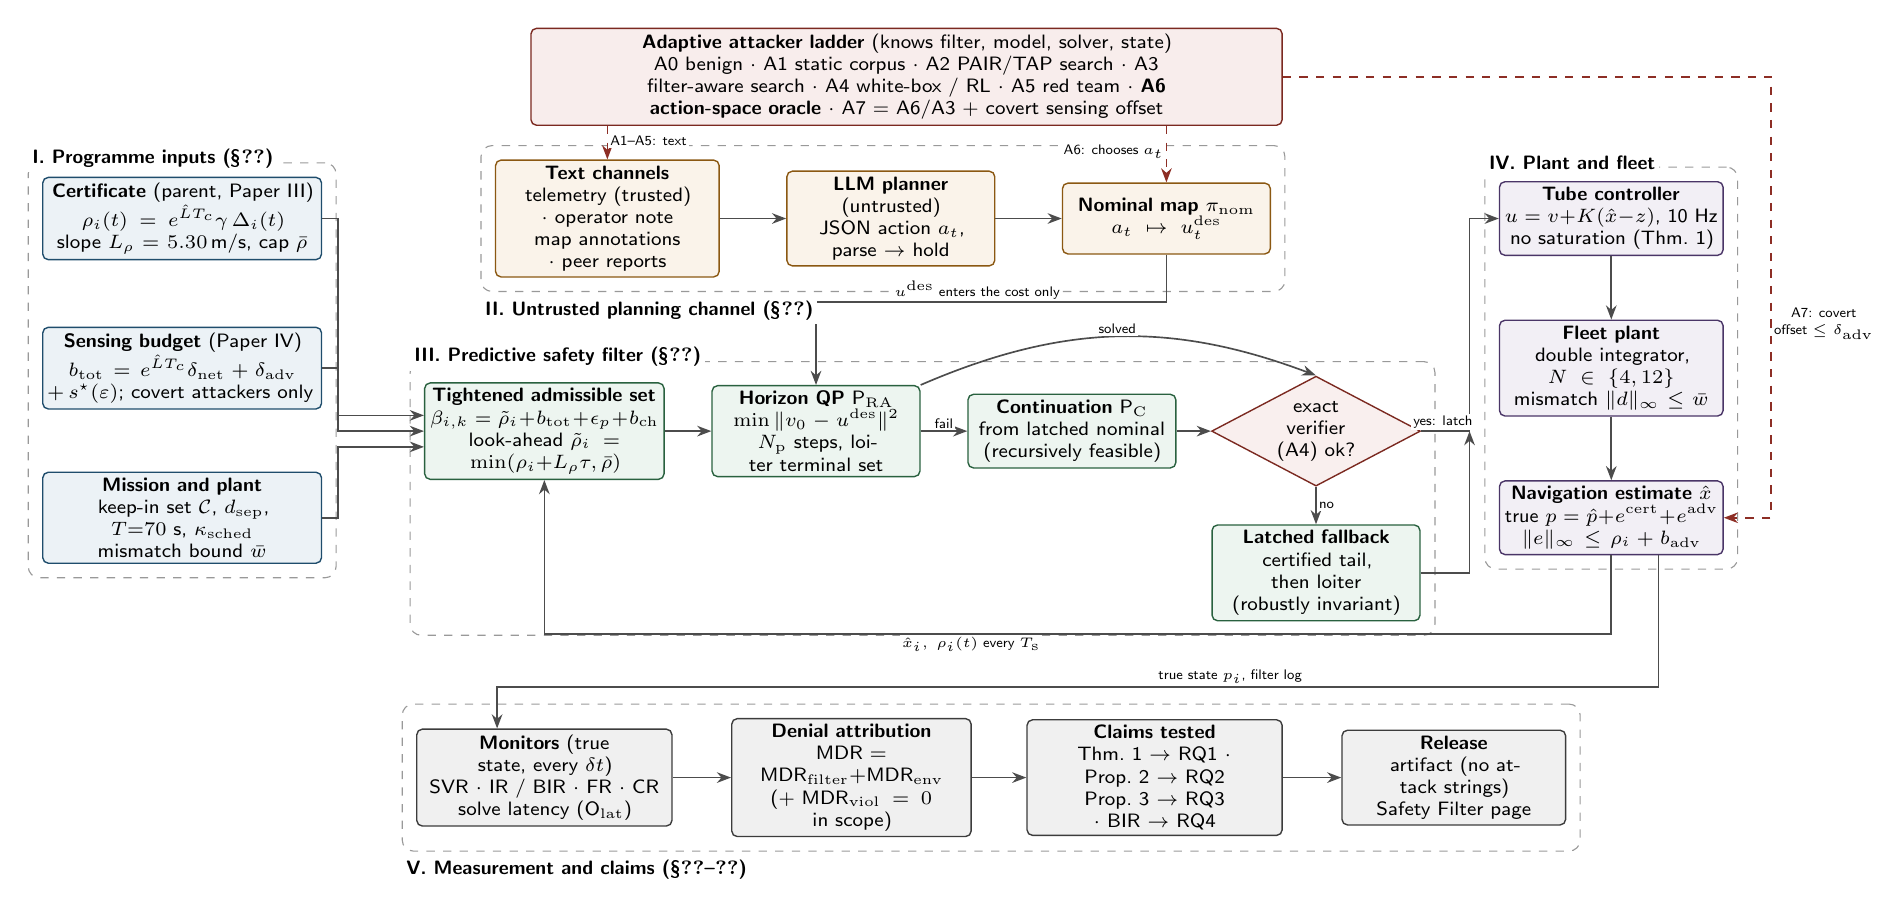
\begin{tikzpicture}[
  font=\sffamily\scriptsize,
  >={Stealth[length=1.8mm]},
  b/.style 2 args={draw=#1!70!black, fill=#1!9, rounded corners=2pt, align=center,
              minimum height=9mm, text width=#2, inner sep=2pt, line width=0.5pt},
  dia/.style={draw=cRed!70!black, fill=cRed!8, diamond, aspect=1.9, align=center,
              inner sep=0pt, text width=12mm, line width=0.5pt},
  phase/.style={draw=black!40, dashed, rounded corners=4pt, inner sep=5pt},
  ptitle/.style={font=\sffamily\bfseries\scriptsize, fill=white, inner sep=1.5pt, anchor=west},
  arr/.style={->, line width=0.6pt, draw=black!70},
  att/.style={->, line width=0.6pt, draw=cRed!80!black, dashed},
  lab/.style={font=\sffamily\tiny, fill=white, inner sep=0.8pt, align=center},
]
% ---------------- Phase I: programme inputs -----------------------------
\node[b={cBlue}{34mm}] (cert) at (-0.15, 0.35)
  {\textbf{Certificate} (parent, Paper III)\\$\rho_i(t)=e^{\hat L T_c}\gamma\,\Delta_i(t)$\\slope $L_\rho=5.30$\,m/s, cap $\bar\rho$};
\node[b={cBlue}{34mm}] (budg) at (-0.15,-1.55)
  {\textbf{Sensing budget} (Paper IV)\\$b_{\mathrm{tot}}=e^{\hat L T_c}\delta_{\mathrm{net}}+\delta_{\mathrm{adv}}$\\$+\,s^\star(\varepsilon)$; covert attackers only};
\node[b={cBlue}{34mm}] (mis) at (-0.15,-3.45)
  {\textbf{Mission and plant}\\keep-in set $\mathcal C$, $d_{\mathrm{sep}}$, $T{=}70$ s, $\kappa_{\mathrm{sched}}$\\mismatch bound $\bar w$};
% ---------------- Adversary ------------------------------------------------
\node[b={cRed}{94mm}] (adv) at (9.05, 2.15)
  {\textbf{Adaptive attacker ladder} (knows filter, model, solver, state)\\
   A0 benign $\cdot$ A1 static corpus $\cdot$ A2 PAIR/TAP search $\cdot$ A3 filter-aware search $\cdot$
   A4 white-box / RL $\cdot$ A5 red team $\cdot$ \textbf{A6 action-space oracle} $\cdot$ A7 = A6/A3 + covert sensing offset};
% ---------------- Phase II: untrusted planning channel -----------------
\node[b={cOrange}{27mm}] (chan) at (5.25, 0.35)
  {\textbf{Text channels}\\telemetry (trusted) $\cdot$ operator note\\map annotations $\cdot$ peer reports};
\node[b={cOrange}{25mm}] (llm) at (8.85, 0.35)
  {\textbf{LLM planner}\\(untrusted)\\JSON action $a_t$, parse $\to$ hold};
\node[b={cOrange}{25mm}] (pin) at (12.35, 0.35)
  {\textbf{Nominal map} $\pi_{\mathrm{nom}}$\\$a_t\mapsto u^{\mathrm{des}}_t$};
\draw[att] (adv.south -| chan.north) -- node[lab, pos=0.45, right] {A1--A5: text} (chan.north);
\draw[att] (adv.south -| pin.north) -- node[lab, pos=0.45, left] {A6: chooses $a_t$} (pin.north);
\draw[arr] (chan) -- (llm);
\draw[arr] (llm) -- (pin);
% ---------------- Phase III: predictive safety filter -------------------
\node[b={cGreen}{29mm}] (adm) at (4.45,-2.35)
  {\textbf{Tightened admissible set}\\$\beta_{i,k}=\tilde\rho_i+b_{\mathrm{tot}}+\epsilon_p+b_{\mathrm{ch}}$\\look-ahead $\tilde\rho_i=\min(\rho_i{+}L_\rho\tau,\bar\rho)$};
\node[b={cGreen}{25mm}] (qp) at (7.9,-2.35)
  {\textbf{Horizon QP} $\mathsf P_{\mathrm{RA}}$\\$\min\|v_0-u^{\mathrm{des}}\|^2$\\$N_{\mathrm p}$ steps, loiter terminal set};
\node[b={cGreen}{25mm}] (cont) at (11.15,-2.35)
  {\textbf{Continuation} $\mathsf P_{\mathrm C}$\\from latched nominal\\(recursively feasible)};
\node[dia] (ver) at (14.25,-2.35) {exact\\verifier\\(A4) ok?};
\node[b={cGreen}{25mm}] (fb) at (14.25,-4.15)
  {\textbf{Latched fallback}\\certified tail, then loiter\\(robustly invariant)};
\draw[arr] (adm) -- (qp);
\draw[arr] (qp) -- node[lab, above] {fail} (cont);
\draw[arr] (cont) -- (ver);
\draw[arr] (qp.north east) to[bend left=22] node[lab, pos=0.5, above] {solved} (ver.north);
\draw[arr] (ver.south) -- node[lab, right] {no} (fb.north);
\draw[arr] (pin.south) -- ++(0,-0.6) -| node[lab, pos=0.27, above] {$u^{\mathrm{des}}$ enters the cost only} (qp.north);
\draw[arr] (cert.east) -- ++(2mm,0) |- ([yshift=2mm]adm.west);
\draw[arr] (budg.east) -- ++(2mm,0) |- (adm.west);
\draw[arr] (mis.east) -- ++(2mm,0) |- ([yshift=-2mm]adm.west);
% ---------------- Phase IV: plant and fleet ------------------------------
\node[b={cPurple}{27mm}] (tube) at (18.0, 0.35)
  {\textbf{Tube controller}\\$u=v+K(\hat x-z)$, 10 Hz\\no saturation (Thm.~1)};
\node[b={cPurple}{27mm}] (plant) at (18.0,-1.55)
  {\textbf{Fleet plant}\\double integrator, $N\in\{4,12\}$\\mismatch $\|d\|_\infty\le\bar w$};
\node[b={cPurple}{27mm}] (est) at (18.0,-3.45)
  {\textbf{Navigation estimate} $\hat x$\\true $p=\hat p+e^{\mathrm{cert}}+e^{\mathrm{adv}}$\\$\|e\|_\infty\le\rho_i+b_{\mathrm{adv}}$};
\draw[arr] (ver.east) -- node[lab, above, pos=0.45] {yes: latch} (16.2,-2.35) |- (tube.west);
\draw[arr] (fb.east) -| (16.2,-2.35);
\draw[arr] (tube) -- (plant);
\draw[arr] (plant) -- (est);
\draw[att] (adv.east) -| node[lab, pos=0.78, right] {A7: covert\\offset $\le\delta_{\mathrm{adv}}$} ([xshift=6mm]est.east) -- (est.east);
\draw[arr] (est.south) -- ++(0,-1.0) -| node[lab, pos=0.3, below] {$\hat x_i,\ \rho_i(t)$ every $T_{\mathrm s}$} (adm.south);
% ---------------- Phase V: monitors, metrics, claims --------------------
\node[b={cGray}{31mm}] (mon) at (4.45,-6.75)
  {\textbf{Monitors} (true state, every $\delta t$)\\SVR $\cdot$ IR / BIR $\cdot$ FR $\cdot$ CR\\solve latency (O$_{\mathrm{lat}}$)};
\node[b={cGray}{29mm}] (attr) at (8.35,-6.75)
  {\textbf{Denial attribution}\\MDR $=$ MDR$_{\mathrm{filter}}+$MDR$_{\mathrm{env}}$\\(+ MDR$_{\mathrm{viol}}=0$ in scope)};
\node[b={cGray}{31mm}] (thy) at (12.2,-6.75)
  {\textbf{Claims tested}\\Thm.~1 $\to$ RQ1 $\cdot$ Prop.~2 $\to$ RQ2\\Prop.~3 $\to$ RQ3 $\cdot$ BIR $\to$ RQ4};
\node[b={cGray}{27mm}] (rel) at (16.0,-6.75)
  {\textbf{Release}\\artifact (no attack strings)\\Safety Filter page};
\draw[arr] ([xshift=6mm]est.south) |- node[lab, pos=0.7, above] {true state $p_i$, filter log} (5.0,-5.6) -| ([xshift=-6mm]mon.north);
\draw[arr] (mon) -- (attr);
\draw[arr] (attr) -- (thy);
\draw[arr] (thy) -- (rel);
% ---------------- phase frames -------------------------------------------
\begin{scope}[on background layer]
\node[phase, fit=(cert)(budg)(mis)] (P1) {};
\node[phase, fit=(chan)(llm)(pin)] (P2) {};
\node[phase, fit=(adm)(qp)(cont)(ver)(fb)] (P3) {};
\node[phase, fit=(tube)(plant)(est)] (P4) {};
\node[phase, fit=(mon)(attr)(thy)(rel)] (P5) {};
\end{scope}
\node[ptitle] at ([yshift=0.5mm]P1.north west) {I.\ Programme inputs (\S\ref{sec:prelim})};
\node[ptitle, anchor=north west] at ([yshift=-0.5mm]P2.south west) {II.\ Untrusted planning channel (\S\ref{sec:threat})};
\node[ptitle] at ([yshift=0.5mm]P3.north west) {III.\ Predictive safety filter (\S\ref{sec:method})};
\node[ptitle] at ([yshift=0.5mm]P4.north west) {IV.\ Plant and fleet};
\node[ptitle, anchor=north west] at ([yshift=-0.5mm]P5.south west) {V.\ Measurement and claims (\S\ref{sec:protocol}--\ref{sec:results})};
\end{tikzpicture}}
\caption{Methodological framework. \textbf{I.} The programme supplies the
navigation certificate $\rho_i(t)$ with its staleness slope $L_\rho$, the
covert sensing budget $b_{\mathrm{tot}}$ and the mission; the plant's
mismatch bound $\bar w$ is new. \textbf{II.} The untrusted LLM planner reads
delimited text channels and emits a JSON action that a fixed nominal map
turns into a desired acceleration $u^{\mathrm{des}}$. Attackers A1--A5 act
through text; the oracle A6 chooses the action directly; A7 adds a covert
sensing offset (dashed red). \textbf{III.} The filter tightens the keep-in
and separation constraints by the look-ahead protection level, the sensing
budget, the mismatch tube and the inter-node chord, then solves a horizon QP
in which $u^{\mathrm{des}}$ enters only the cost. If the re-anchored problem
fails, a continuation problem from the latched nominal is solved. Only plans
that an exact verifier accepts are latched; otherwise the fleet continues the
last certified plan and then loiters. \textbf{IV.} A tube controller tracks
the latched nominal. \textbf{V.} Monitors evaluate the \emph{true} state at
every plant step and attribute every denied mission to the filter or to the
planner; the measurements test Theorem~1 and Propositions~2--3 and answer
RQ1--RQ4.}
\label{fig:framework}
\end{figure*}

% =====================================================================
\section{The Predictive Safety Filter and Its Guarantees}\label{sec:method}
% =====================================================================
\subsection{Two time scales and the tube controller}
The filter runs every $\Ts=S\,\delta t$ (in the pilot $\delta t=0.1$\,s,
$\Ts=0.5$\,s, $S=5$). It plans a nominal trajectory $z_{i,k}=(p(z_{i,k}),\mathrm{vel}(z_{i,k}))$
over $\Np$ intervals with piecewise-constant nominal accelerations $v_{i,k}$:
\begin{equation}\label{eq:nominal}
z_{i,k+1}=A_{\mathrm s}z_{i,k}+B_{\mathrm s}v_{i,k},\quad A_{\mathrm s}=\left[\begin{smallmatrix}1&\Ts\\0&1\end{smallmatrix}\right],\ B_{\mathrm s}=\left[\begin{smallmatrix}\Ts^2/2\\\Ts\end{smallmatrix}\right].
\end{equation}
Between ticks, a tube controller tracks the latched nominal $z(n)$ on the
fine grid,
\begin{equation}\label{eq:tube}
u_i(n)=v_i(n)+K\bigl(\hat x_i(n)-z_i(n)\bigr),
\end{equation}
with $K=-[k_p\ \ k_d]=-[1.2\ \ 1.8]$.
The gains are Paper~IV's lateral PD gains~\cite{paperIV}. The tracking error
$\xi_i=\hat x_i-z_i$ obeys $\xi_i(n{+}1)=\Phi\,\xi_i(n)+B_\delta d_i(n)$ with
$\Phi=A_\delta+B_\delta K$, whose spectral radius is $\lambda_c=0.909$. After $n$
steps from an anchor where $\xi=0$, the per-axis error is bounded by the
reachable-set sums
\begin{equation}\label{eq:eps}
\epsilon_\star(n)=\wbar\textstyle\sum_{q=0}^{n-1}|c_\star\Phi^qB_\delta|,\quad c_p=e_1^\top,\ c_v=e_2^\top,\ c_u=K,
\end{equation}
which converge because $\Phi$ is Schur. This is a Chisci-type
tightening~\cite{chisci2001} for a tube controller~\cite{mayne2005tube}; like
the contraction-based tightening of K\"ohler
et~al.~\cite{kohler2021robust}, it stays bounded in the horizon. The
Lipschitz-based alternative~\cite{limon2002iss} grows geometrically. At
$\wbar=0.5$\,m/s$^2$: $\epsilon_p(\infty)=0.424$\,m,
$\epsilon_v(\infty)=0.400$\,m/s and $\epsilon_u(\infty)=0.690$\,m/s$^2$. The
nominal acceleration is therefore limited to
$\unom=\umax-\epsilon_u(\infty)=3.310$\,m/s$^2$, which guarantees that
\cref{eq:tube} never saturates.

\subsection{Constraint tightening}\label{sec:tightening}
Consider a plan created at tick $t_j$ whose tube was last anchored $a$ fine
steps earlier ($a=0$ for a plan that starts at the navigation state). Using
Paper~III's look-ahead~\cite{paperIII}, the predicted protection level is
\begin{equation}\label{eq:lookahead}
\tilde\rho_i(t_j;\tau)=\min\bigl\{\max\{\rho_i(t_j),\rhofl\}+\Lrho\tau,\ \rhobar\bigr\}.
\end{equation}
It covers growth at slope $\Lrho$, a re-anchor to at most $\rhofl$ within
the horizon, and the cap $\rhobar$. The per-axis tightening at node $k$ is
\begin{equation}\label{eq:beta}
\beta_{i,k}=
\begin{cases}
\tilde\rho_{i,k}+\btot+\epsilon_{p,k}+\bch, & k<\Np,\\
\rhobar+\btot+\epsilon_p(\infty)+\bch, & k=\Np,
\end{cases}
\end{equation}
with $\tilde\rho_{i,k}=\tilde\rho_i(t_j;(k{+}1)\Ts)$ and $\epsilon_{p,k}=\epsilon_p(a+(k{+}1)S)$,
and $\bch=\unom\Ts^2/8$ bounds the deviation of the nominal path from the
chord between two nodes. Every term is non-decreasing in $k$, so
$\beta_{i,k}$ covers the whole interval that follows node $k$. Node
constraints use $\hat\beta_{i,0}=\beta_{i,0}$ and
$\hat\beta_{i,k}=\max\{\beta_{i,k-1},\beta_{i,k}\}$, so that both ends of
every interval are tightened for that interval. Speeds are tightened by
$\epsilon_v$ and inputs by $\epsilon_u(\infty)$. At $\btot=4.371$\,m the
terminal tightening is 9.898\,m.

\subsection{The filter problem}
At tick $t_j$, with start state $\zeta_i$ and tube age $a$, the filter solves
\begin{subequations}\label{eq:qp}
\begin{align}
\min_{\{v_{i,k}\}}\ & \textstyle\sum_{i}\|v_{i,0}-\uDes_i\|_2^2+\mu\sum_{i}\sum_{k=1}^{\Np-1}\|v_{i,k}\|_2^2 \label{eq:qp-cost}\\
\text{s.t.}\ & z_{i,0}=\zeta_i,\quad z_{i,k+1}=A_{\mathrm s}z_{i,k}+B_{\mathrm s}v_{i,k},\label{eq:qp-dyn}\\
& h_r^\top p(z_{i,k})\le c_r-\|h_r\|_1\hat\beta_{i,k}\quad \forall r,\ k=0,\dots,\Np,\label{eq:qp-cor}\\
& n_{il,k}^\top\bigl(p(z_{i,q})-p(z_{l,q})\bigr)\notag\\
& \qquad\ge\dsep+\|n_{il,k}\|_1\bigl(\bar\beta_{i,kq}+\bar\beta_{l,kq}\bigr),\ q\in\{k,k{+}1\},\label{eq:qp-sep}\\
& |v_{i,k}|\le\unom,\quad |\mathrm{vel}(z_{i,k})|\le\vmax-\epsilon_{v,k}^{+},\label{eq:qp-box}\\
& \mathrm{vel}(z_{i,\Np})=0\qquad\text{(loiter terminal set)},\label{eq:qp-term}
\end{align}
\end{subequations}
for all $i<l$ and $k<\Np$ in \eqref{eq:qp-sep}, with $\bar\beta_{i,kq}=\max\{\beta_{i,k},\beta_{i,q}\}$, $\epsilon_{v,k}^{+}=\epsilon_v(a+\min\{k{+}1,\Np\}S)$ and $\mu=10^{-4}$.
The separation constraint is a linearisation along a unit normal $n_{il,k}$
taken from a reference trajectory. For any unit normal it implies
$\|p_i-p_l\|_2\ge n^\top(p_i-p_l)$, so it is conservative. Constraint
\eqref{eq:qp-sep} is imposed at both ends of every interval with the same
normal, so it holds along the whole relative chord. The planner's proposal
enters \eqref{eq:qp} \emph{only} through $\uDes$ in the cost. The feasible
set does not depend on it, and this is the structural fact behind the
quantifier ``for every planner''.

\paragraph{Re-anchoring, continuation and fallback} Each tick runs up to
three stages (\cref{alg:filter}).
\begin{enumerate}
\item \textbf{Re-anchored problem} $\PRA$: start at
  the navigation state, $\zeta_i=\hat x_i(t_j)$, with tube age $a=0$, and
  normals from the latched plan shifted to the current state.
\item \textbf{Continuation problem} $\PC$: if $\PRA$ fails, start from the
  latched nominal state, $\zeta_i=z_i^{\mathrm{lat}}(t_j)$, with the
  accumulated tube age and the latched plan's own normals, shifted by one
  tick.
\item \textbf{Fallback}: if both fail, execute the remaining tail of the
  latched certified plan, then loiter at its terminal node.
\end{enumerate}
Only stage~3 counts as a fallback. Every candidate plan is re-simulated and
checked by an independent evaluator that uses exact arithmetic and none of
the solver's numerical buffers. A plan that fails this check is treated as a
solver failure. Re-anchoring alone does not preserve recursive feasibility
under worst-case disturbance near the boundary: the new tightening counts
error that has already been realised. The continuation problem is the
remedy, in the spirit of tube MPC with a free initial nominal
state~\cite{mayne2005tube}. Black-box Simplex~\cite{mehmood2022bbsimplex}
supplies the idea of keeping the last valid certificate.

\begin{algorithm}[t]
\caption{One filter tick at $t_j$ (all aircraft jointly)}\label{alg:filter}
\begin{algorithmic}[1]
\State $\uDes\gets\pinom(\hat x,a_t)$ \Comment{untrusted input, cost only}
\State $(\mathit{ok},V)\gets$ solve $\PRA$ from $\hat x(t_j)$, age $0$; verify exactly
\If{not $\mathit{ok}$ and a certified latched plan exists}
  \State $(\mathit{ok},V)\gets$ solve $\PC$ from $z^{\mathrm{lat}}(t_j)$, age $a^{\mathrm{lat}}$; verify
\EndIf
\If{$\mathit{ok}$} latch $(z,V)$ \Comment{certified, executed by \eqref{eq:tube}}
\Else\ keep latched plan; its tail, then loiter \Comment{fallback}
\EndIf
\end{algorithmic}
\end{algorithm}

\subsection{Theorem 1: planner-invariant robust safety}\label{sec:thm1}
\begin{assumption}[Bounded mismatch]\label{as:mismatch}
$\|d_i(n)\|_\infty\le\wbar$ for all $i,n$ in \eqref{eq:plant}.
\end{assumption}
\begin{assumption}[Sound, rate-bounded certificate; covert budget]\label{as:cert}
$\|e^{\mathrm{cert}}_i(n)\|_\infty\le\rho_i(t_n)$. Between re-anchors,
$\rho_i$ grows at most at slope $\Lrho$; a re-anchor resets it to at most
$\rhofl$; and $\rho_i\le\rhobar$ always, with no jumps ($\bar J=0$, the
delay-adversary regime). The sensing offset satisfies
$\|e^{\mathrm{adv}}_i\|_\infty\le\badv\le\btot$ (Paper~IV's covert class).
\end{assumption}
\begin{assumption}[Well-posed tightening]\label{as:wellposed}
$\Phi$ is Schur, $\epsilon_u(\infty)<\umax$ and $\epsilon_v(\infty)<\vmax$.
\end{assumption}
\begin{assumption}[Verified execution]\label{as:verified}
A plan is latched only after an independent evaluator has checked every
constraint of \eqref{eq:qp} on its rollout. Solver failure, time-out or a
failed check is reported as failure and never executes.
\end{assumption}
\begin{assumption}[Initial certification]\label{as:init}
At $t_0$ the problem $\PRA$ has a verified solution.
\end{assumption}

\begin{theorem}[Planner-invariant robust safety]\label{thm:safety}
Let \cref{as:mismatch,as:cert,as:wellposed,as:verified,as:init} hold.
Consider every planner: any, possibly randomised, map from the full history
(including the filter's internal state, the solver, the certificate, the
disturbance and the sensing offset) to action sequences. Consider also every
disturbance allowed by \cref{as:mismatch} and every certificate and offset
trajectory allowed by \cref{as:cert}. Then, at every plant step $n$ and for
all $i\neq l$:
\begin{enumerate}[label=(\roman*)]
\item the true position satisfies $p_i(n)\in\Cset$;
\item $\|p_i(n)-p_l(n)\|_2\ge\dsep$;
\item $|u_i(n)|\le\umax$ and $|\hat v_i(n)|\le\vmax$, so the actuators never saturate;
\item whenever a certified plan is latched at $t_j$, $\PC$ is feasible at
  $t_{j+1}$, so a fallback can only follow a solver or verifier failure, never
  infeasibility; a fallback preserves (i)--(iii) indefinitely.
\end{enumerate}
\end{theorem}

The proof rests on three lemmas. Full index bookkeeping is in
\cref{app:proofs}.

\begin{lemma}[Tube]\label{lem:tube}
If $\xi_i=0$ at an anchor and \eqref{eq:tube} tracks a nominal trajectory that
is continuous across ticks, then $n$ steps later
$|e_1^\top\xi_i|\le\epsilon_p(n)$, $|e_2^\top\xi_i|\le\epsilon_v(n)$ and
$|K\xi_i|\le\epsilon_u(n)$ per axis, provided no saturation occurs.
\end{lemma}
\begin{proof}
Without saturation, $\xi_i(n)=\sum_{q=0}^{n-1}\Phi^qB_\delta d_i(n{-}1{-}q)$.
Apply the triangle inequality with $|d_i|\le\wbar$ per axis. The dynamics
decouple per axis.
\end{proof}

\begin{lemma}[A certified plan is safe while followed]\label{lem:certplan}
Let a plan be verified at $t_j$ from start $\zeta$ with tube age $a$, where
$|\xi(t_j)|$ is bounded by the tube at age $a$. Suppose the plan is followed
by \eqref{eq:tube} and then held at its terminal node with $v=0$ for any
length of time. Then (i)--(iii) hold at every step of that execution.
\end{lemma}
\begin{proof}
Take a step $n$ in interval $k$, so $t_j+k\Ts\le t_n\le t_j+(k{+}1)\Ts$. By
\eqref{eq:truepos}, $p_i(n)=z_i(n)+e_1^\top\xi_i(n)+e^{\mathrm{cert}}_i(n)+e^{\mathrm{adv}}_i(n)$.
Each axis of $z_i(n)$ lies within $\bch$ of the chord point between
$p(z_{i,k})$ and $p(z_{i,k+1})$, because the nominal acceleration is bounded by
$\unom$ (\cref{as:verified} enforces \eqref{eq:qp-box}). By \cref{lem:tube}
and monotonicity, $|e_1^\top\xi_i(n)|\le\epsilon_p(a+(k{+}1)S)$.

By \cref{as:cert}, $\rho_i(t_n)\le\tilde\rho_i(t_j;(k{+}1)\Ts)$. If no re-anchor
occurs in $[t_j,t_n]$, $\rho_i$ grows by at most $\Lrho(t_n-t_j)$. If one
occurs at time $s$, then $\rho_i(t_n)\le\rhofl+\Lrho(t_n-s)$. In both cases
the cap is $\rhobar$. Hence every axis of $p_i(n)$ lies within $\beta_{i,k}$
of the chord point.

Both chord endpoints satisfy \eqref{eq:qp-cor} with
$\hat\beta\ge\beta_{i,k}$, and the half-space $\{y:h_r^\top y\le
c_r-\|h_r\|_1\beta_{i,k}\}$ is convex. The chord point therefore satisfies it,
and $h_r^\top p_i(n)\le h_r^\top(\text{chord})+\|h_r\|_1\beta_{i,k}\le c_r$:
claim~(i). Separation follows in the same way. The constraint
\eqref{eq:qp-sep} holds at both ends of the interval with the same $n_{il,k}$
and with $\bar\beta\ge\beta_{\cdot,k}$, so it holds on the relative chord. The
relative deviation is at most $\|n\|_1(\beta_{i,k}+\beta_{l,k})$ along $n$, and
$\|p_i-p_l\|_2\ge n^\top(p_i-p_l)\ge\dsep$: claim~(ii).

For claim~(iii), the nominal velocity is affine within an interval, so it is
bounded by its node values; together with $|e_2^\top\xi|\le\epsilon_v$ this
gives $|\hat v_i|\le\vmax$. Also $|u|\le|v|+|K\xi|\le\unom+\epsilon_u(\infty)=\umax$,
which also justifies the no-saturation premise of \cref{lem:tube} by
induction over steps.

After the horizon, the nominal rests at $z_{i,\Np}$, $|\xi|\le\epsilon(\infty)$
and $\rho_i\le\rhobar$. These are covered by $\beta_{i,\Np}$ and by the
terminal-node constraints: the loiter set is robustly invariant.
\end{proof}

\begin{lemma}[Shift feasibility of the continuation problem]\label{lem:shift}
Suppose a plan $(z,v)$ with normals $n_{\cdot,k}$ is certified at $t_j$ with
age $a$. At $t_{j+1}$, take the shifted candidate $z'_k=z_{k+1}$ and
$z'_{\Np}=z_{\Np}$, with $v'_k=v_{k+1}$ for $k<\Np-1$ and $v'_{\Np-1}=0$, and
normals $n'_k=n_{\min\{k+1,\Np-1\}}$, at age $a+S$. This candidate is feasible
for $\PC$.
\end{lemma}
\noindent The proof is index bookkeeping: tube terms match by an index
shift, \cref{as:cert} makes the shifted look-ahead no larger, and the
appended node is the old terminal node at rest (\cref{app:proofs}).

\begin{proof}[Proof of \cref{thm:safety}]
We argue by induction over ticks. The invariant $\mathcal I_j$ is: \emph{at
$t_j$ a certified plan is latched, and its continued execution followed by
loitering satisfies (i)--(iii)}. $\mathcal I_0$ holds by \cref{as:init} and
\cref{lem:certplan}.

Assume $\mathcal I_j$. At $t_{j+1}$ exactly one of three events occurs:
\begin{itemize}
\item $\PRA$ returns a verified plan. Its start is the navigation state,
  so $\xi=0$ and the tube age is 0; \cref{lem:certplan} applies.
\item $\PC$ returns a verified plan. Its start is the latched nominal state,
  which is continuous with the executed nominal, so $\xi(t_{j+1})$ is bounded
  by the tube at the accumulated age; \cref{lem:certplan} applies again.
\item Neither returns a verified plan. The old plan stays latched and
  $\mathcal I_j$ carries over unchanged.
\end{itemize}
In every case $\mathcal I_{j+1}$ holds, which proves (i)--(iii).

\Cref{as:verified} excludes any fourth event, such as an unverified plan
being executed. The case analysis never refers to $\uDes$: the planner enters
only the cost of \eqref{eq:qp}, which selects \emph{among} verified plans. The
statement therefore holds uniformly over all planners, including adaptive
ones that know the filter. Claim~(iv) is \cref{lem:shift} combined with the
third case.
\end{proof}

\paragraph{Why this is more than recursive feasibility} The machinery is
that of predictive safety
filters~\cite{wabersich2021psf,wabersich2023datadriven,rawlings2017mpc}, but
the constraint set is exogenous and driven by an adversarial certificate
process, the guarantee concerns a state the filter never observes (the true
position), and the quantifier ranges over adversarial, history-dependent
planners rather than an imperfect learner. FaSTrack's planner-agnostic
tracking bound~\cite{herbert2017fastrack} has the same quantifier structure
for references. The guarantee is stated at plant sampling instants; a
continuous-time claim needs an additional inter-sample margin.

\subsection{Transparency}
\begin{lemma}[Transparency]\label{lem:transparent}
Let $\Aadm(\zeta)=\{v_0:\exists$ a feasible plan of \eqref{eq:qp} with first
input $v_0\}$.
\begin{enumerate}[label=(\alph*)]
\item If $\uDes\notin\Aadm$, the filter intervenes ($v^\star_0\neq\uDes$).
\item If $\uDes\in\Aadm$ and $\mu=0$, the filter returns $\uDes$ unchanged.
\item For $\mu>0$, the deviation is at most
  $\|v^\star_0-\uDes\|_2^2\le2\mu N(\Np{-}1)\unom^2$.
\end{enumerate}
\end{lemma}
\begin{proof}
For (a), no feasible plan starts with $\uDes$. For (b), the cost is minimised
at $\uDes$ over a set that contains it. For (c), compare with the feasible plan
that starts with $\uDes$: its cost is at most $\mu$ times the squared norm of a
tail that \eqref{eq:qp-box} bounds.
\end{proof}

Interventions are therefore forced only when a proposal leaves the
admissible set of the \emph{tightened} problem. The benign intervention rate
(BIR) measures two things together: how unsafe the planner's proposals are,
and the conservatism gap between the maximal robust invariant set and the
tightened feasible set. That gap shrinks as $\wbar\to0$ and as $\Np$ grows.

\subsection{Proposition 2: safety confinement and the denial taxonomy}
For aircraft $i$, let $g_i(t_j)$ be the unit vector towards its goal, and let
$v^{\mathrm{req}}_i(t_j)$ be the velocity its action asks for: the commanded
velocity for \code{goto} and \code{velocity}, the braking target for
\code{hold}, and $\hat v_i+a\cdot1$\,s for an acceleration-mode oracle
action. Define the \emph{progress intent} accumulated before the deadline,
\begin{equation}\label{eq:intent}
I_i=\textstyle\sum_{t_j<(1+\ksched)T}\max\{\langle v^{\mathrm{req}}_i(t_j),g_i(t_j)\rangle,0\}\,\Ts .
\end{equation}
Let $D_i$ be the initial goal distance minus the goal radius. A denied
mission is \emph{filter-induced} if some aircraft missed the deadline even
though $I_i\ge D_i$. That is, the planner asked for enough progress and the
filter's interventions or fallbacks prevented it. Otherwise the denial is
\emph{in-envelope}: the planner never asked for enough.

\begin{proposition}[Safety/liveness split]\label{prop:liveness}
Under the assumptions of \cref{thm:safety}, the following holds for every
attacker in the ladder.
\begin{enumerate}[label=(\alph*)]
\item \emph{Confinement:} $\Pr[\sigma\in S]=1$. The attacker's only
  achievable objectives are traces in $S\setminus L$ (denial), stealth
  within $S$, or breaking an assumption.
\item \emph{Decomposition:} $\MDR=\MDR_{\mathrm{filter}}+\MDR_{\mathrm{env}}+\MDR_{\mathrm{viol}}$
  with $\MDR_{\mathrm{viol}}=0$. The two remaining terms partition the denied
  missions.
\item \emph{In-envelope denial is invisible to any transparent filter:}
  let $\mathcal F$ be any filter (ours or another) that returns unchanged
  every proposal in a set $\mathcal A_0$. Then a planner whose proposals stay
  in $\mathcal A_0$ yields the same executed action stream with and without
  $\mathcal F$. Its denial is filter-invariant, so $\mathcal F$ cannot reduce
  the $\MDR_{\mathrm{env}}$ that such planners cause. In particular, a filter
  that admits its own fallback action (hold or loiter) admits a planner that
  proposes only that action.
\end{enumerate}
\end{proposition}
\begin{proof}
(a)~is \cref{thm:safety}. (b)~holds by definition, because the two classes
are complementary on denied missions without violations. (c)~By hypothesis,
$\mathcal F(a)=a$ for every $a\in\mathcal A_0$, so the action streams coincide
pathwise, and so does any mission outcome determined by them. For our
filter, \cref{lem:transparent}(b) identifies $\mathcal A_0$ with
$\Aadm$.
\end{proof}

Part~(c) is structural: it does not depend on how the filter is tuned. A
physical filter guards the envelope, and an attacker that stays inside the
envelope is not its business. Looping or ``malfunction amplification''
attacks on LLM agents~\cite{zhang2024breakingagents} are exactly this class.
Filter-induced denial has its own control-theoretic mechanism. Minimally
invasive barrier filters create asymptotically stable spurious equilibria
on the boundary of the safe set~\cite{reis2021undesired} and deadlock in
multi-robot settings~\cite{grover2020deadlock}. An attacker that rides the
boundary exploits exactly these equilibria. Stealth is a third dimension, not
a third term: it is any denial trace whose per-step anomaly signals stay below
an operator's threshold. RL-Hammer reaches 0\% detection with 97\% ASR on the
language channel~\cite{wen2025rlhammer}.

\subsection{Proposition 3: nestedness under the sensing budget}
\begin{proposition}[Nested admissible sets]\label{prop:nested}
Fix $\zeta$, $\rho$, the tube age and the normals, and let $b\le b'$. Then:
\begin{enumerate}[label=(\alph*)]
\item the feasible set of \eqref{eq:qp} at $b'$ is contained in that at $b$,
  hence $\Aadm(\zeta;b')\subseteq\Aadm(\zeta;b)$;
\item the optimal cost satisfies $J^\star(b')\ge J^\star(b)$, and the
  one-step intervention indicator is monotone:
  $\mathbf 1[\uDes\notin\Aadm(b)]\le\mathbf 1[\uDes\notin\Aadm(b')]$;
\item the same nestedness holds in $\rho$, $\wbar$, $\gamma$ (through $\Lrho$
  and $\rhobar$) and $\bar\Delta$;
\item $\btot(\varepsilon)$ in \eqref{eq:btot} is non-increasing in $\varepsilon$,
  non-decreasing in $\dnet$ and $\dadv$, and non-decreasing under first-order
  stochastic dominance of any benign marginal.
\end{enumerate}
\end{proposition}
\begin{proof}
(a)~$\btot$ enters \eqref{eq:beta} additively, and $\beta$ enters
\eqref{eq:qp-cor} and \eqref{eq:qp-sep} only through right-hand sides of the
form $c-\alpha\beta$ and $d+\alpha\beta$ with $\alpha\ge0$. Increasing $b$
therefore shrinks every constraint set while leaving the dynamics unchanged.
(b)~A minimum over a smaller set is no smaller, and (b) restates (a)
pointwise. (c)~$\tilde\rho$, $\epsilon_{p,v,u}$ and $\rhobar$ are
non-decreasing in these parameters ($\epsilon$ is linear in $\wbar$).
(d)~$\bar p$ is non-increasing, so $s^\star$ is non-increasing in
$\varepsilon$. Deterministic terms shift the margin (Paper~IV,
Prop.~2(e)~\cite{paperIV}). A tail of a sum is non-decreasing under
first-order stochastic dominance of a summand, for every coupling (proof of
Paper~IV, Thm.~1).
\end{proof}

\paragraph{What is not claimed} \Cref{prop:nested} is pointwise. Pathwise
monotonicity of the \emph{rate} of intervention, fallback or denial in
$\btot$ does not follow, because closed-loop trajectories diverge as $b$
changes. We therefore state it as a hypothesis,
\textbf{H3}: \emph{the closed-loop $\IR$, $\FR$ and $\MDR$ are non-decreasing
in $\btot$}. We test it with ordered-trend tests under common random numbers
(CRN) (\cref{sec:rq3}). Composition is only meaningful for Paper~IV's covert
class. A detection-indifferent spoofer that drives the estimator outside
\cref{as:mismatch,as:cert} is the stealthy-deactivation
attack~\cite{arnstrom2024stealthy}. In the terms of Paper~II's runtime
assurance lift $L_{\mathrm{mon}}$~\cite{paperII}, this is where monitor
independence fails.

\begin{remark}[What is \emph{not} guaranteed]\label{rem:notguaranteed}
\begin{enumerate}[label=(\roman*)]
\item \emph{Liveness.} Persistent denial is possible by
  \cref{prop:liveness}(c).
\item \emph{Estimator attacks.} Attacks that move $\hat x$ beyond $\wbar$, or
  falsify $\rho_i$, void \cref{as:mismatch} or \cref{as:cert}.
\item \emph{Certificate jumps.} Relay jumps beyond $\rhobar$ void
  \cref{as:cert}. The median two-hop jump, about 41.8\,m, exceeds every
  margin in the programme's family $\{2,5,10,20\}$\,m. There the theorem is
  \emph{silent}, as the parent certificate is silent outside its own scope
  conditions.
\item \emph{An empty admissible set at take-off.} If \cref{as:init} fails,
  the filter must refuse dispatch. Anything flown after that is uncertified.
\item \emph{Model transfer.} The guarantee concerns the model
  \eqref{eq:plant}. On hardware, $\wbar$ must be identified, not assumed; and
  $\gamma$ was measured in hover~\cite{parentpaper}.
\end{enumerate}
\end{remark}

% =====================================================================
\section{Adaptive Evaluation Protocol}\label{sec:protocol}
% =====================================================================
A defence evaluated against a fixed attack proves
little~\cite{carlini2017towards,athalye2018obfuscated,tramer2020adaptive,carlini2019evaluating}.
We carry the adaptive-evaluation discipline to the physical layer and add
one advantage that model-level defences lack: because \cref{thm:safety} is a
statement over \emph{all} action sequences, the strongest attacker for the
safety claim needs no language model at all.

\subsection{Attacker ladder}
\Cref{tab:ladder} lists the eight levels. Each level is a superset of the
one before it, and every level reports violations and denial against the
four goals G1--G4.

\begin{table}[t]
\centering\scriptsize
\caption{Attacker ladder. A6 needs no LLM and upper-bounds A1--A5 for the
safety claim (\cref{cor:oracle}). Status refers to this paper.}
\label{tab:ladder}
\setlength{\tabcolsep}{2.5pt}
\begin{tabularx}{\columnwidth}{@{}l>{\raggedright\arraybackslash}X>{\raggedright\arraybackslash}p{19mm}@{}}
\toprule
Lvl & Capability and construction & Status \\
\midrule
A0 & Benign scripted mission planner & pilot (scripted) \\
A1 & Static injection corpus: AgentDojo ``important message''~\cite{debenedetti2024agentdojo}, InjecAgent~\cite{zhan2024injecagent}, HouYi~\cite{liu2023houyi}, translated to mission text & \pending \\
A2 & Black-box, filter-unaware LLM search (PAIR/TAP~\cite{chao2025pair,mehrotra2024tap}) & \pending \\
A3 & Black-box, filter-aware: knows the constraint set, observes the intervene bit; cross-entropy method (CEM)~\cite{rubinstein2004cem} or covariance matrix adaptation (CMA-ES)~\cite{hansen2016cma} over template parameters & \pending \\
A4 & White-box open-weights planner: greedy coordinate gradient (GCG)~\cite{zou2023universal} or reinforcement learning (RL)~\cite{wen2025rlhammer} with a stealth reward & \pending\ (optional) \\
A5 & Human red team~\cite{nasr2026attacker} & \pending\ (optional) \\
A6 & \textbf{Action-space oracle}: chooses $\aLLM$ directly; CEM-tuned and hand-designed push families, with worst-case nature & pilot \\
A7 & A6 or A3 composed with Paper~IV's covert sensing offset & pilot (offset realised at budget); detector-gated version \pending \\
\bottomrule
\end{tabularx}
\end{table}

\paragraph{Oracle family used in the pilot} For each aircraft, the oracle
proposes the acceleration $\umax\,\mathrm{dir}/\|\mathrm{dir}\|_\infty$, where
\begin{equation*}
\mathrm{dir}=w_{\mathrm{wall}}h_{r^\star}+w_{\mathrm{nbr}}\hat n_{\mathrm{nn}}+w_{\mathrm{c}}(\cos\phi,\sin\phi)+w_{\mathrm{vel}}\hat v+w_{\mathrm{goal}}\hat g .
\end{equation*}
Here $h_{r^\star}$ is the normal of the most binding wall and $\hat n_{\mathrm{nn}}$
points to the nearest neighbour. The filter returns the minimum-deviation
admissible input, so a maximal push towards a constraint is already the
filter-aware one-step optimum: the filtered input rides the boundary of the
tightened set. CEM tunes the mixture
$\theta=(w_{\mathrm{wall}},w_{\mathrm{nbr}},w_{\mathrm c},\phi,w_{\mathrm{vel}},w_{\mathrm{goal}})$
over whole closed-loop episodes with the filter in the loop. The
\emph{violation} oracle minimises the closest true approach to any
constraint. The \emph{denial} oracle maximises missed deadlines plus fallback
and intervention fractions, but its search box forces
$w_{\mathrm{goal}}\ge0.5$. It is an attacker that wants the \emph{filter} to
cause the denial. Nature is adversarial in both: the disturbance, the
certificate error and the sensing offset all point at each aircraft's most
binding constraint. This box worst case is exactly what the
$\|h\|_1$-scaled tightening covers.

\begin{corollary}[Oracle envelope]\label{cor:oracle}
Let $\Pi_k$ be the set of causal action policies that a language-mediated
attacker at level $k\in\{1,\dots,5\}$ can induce through any text, and let
$\Pi_{\mathrm{act}}$ be all causal action policies (A6). Then
$\Pi_k\subseteq\Pi_{\mathrm{act}}$. Hence:
\begin{enumerate}[label=(\alph*)]
\item $\sup_{\Pi_k}\SVR\le\sup_{\Pi_{\mathrm{act}}}\SVR=0$ under the
  assumptions of \cref{thm:safety};
\item for any liveness metric $M\in\{\MDR,\FR,\IR\}$,
  $\sup_{\Pi_k}M\le M^\star_{\mathrm{A6}}\coloneqq\sup_{\Pi_{\mathrm{act}}}M$.
\end{enumerate}
\end{corollary}
\begin{proof}
The planner's output is restricted to the action schema, so every text
attack induces some action policy. The rest follows from
\cref{thm:safety} and from monotonicity of the supremum.
\end{proof}

The searched oracle achieves $M_{\mathrm{A6}}^{\mathrm{search}}\le M^\star_{\mathrm{A6}}$,
so for liveness it is a lower bound on the oracle's power, not a proof of the
strongest attack. We call
$M_{\mathrm{A6}}^{\mathrm{search}}-\max_{k\le5}M(\mathrm A_k)$ the
\emph{LLM-mediation slack}. It measures how much of the theoretically
available denial an attacker can actually realise through text.

\paragraph{Sanity checks}
Following Carlini et~al.~\cite{carlini2019evaluating}:
\begin{enumerate}[label=(\roman*)]
\item with the filter off, attacks must produce violations; otherwise they
  are too weak to say anything;
\item an unbounded oracle must reach near-total denial;
\item attack success must not decrease with search budget;
\item results are the \emph{worst case over attackers per mission}, never an
  average over attacks.
\end{enumerate}

\subsection{Metrics}\label{sec:metrics}
We follow AgentDojo's split into benign utility, utility under attack and
targeted ASR~\cite{debenedetti2024agentdojo}, and Paper~III's per-step
counting convention~\cite{paperIII}. Let $n_{\mathrm{st}}$ be the number of
plant steps and $n_{\mathrm{tk}}$ the number of filter ticks of an episode.
\begin{itemize}
\item \textbf{Safety-violation rate}
  $\SVR=\#\{(i,n):p(n)\notin\mathcal S\text{ through }i\}/(N\,n_{\mathrm{st}})$,
  counted per aircraft-step and never averaged per episode. Here $\SVR$
  answers RQ1.
\item \textbf{Intervention rate}
  $\IR=\#\{(i,j):\|v^\star_{i,0}-\uDes_i\|_\infty>\eta\}/(N\,n_{\mathrm{tk}})$,
  with $\eta=0.01$\,m/s$^2$; it includes fallback ticks. $\BIR$ is $\IR$
  under A0.
\item \textbf{Fallback rate} $\FR$: the fraction of fleet ticks that
  execute the latched tail. \textbf{Continuation rate} $\CR$: the fraction of
  ticks certified by $\PC$.
\item \textbf{Mission completion and denial} $\MCR$ and $\MDR$ follow
  \eqref{eq:mcr} with $\ksched=0.10$ (headline) and $0.25$ (sensitivity),
  with the split of \cref{prop:liveness}.
\item \textbf{Benign mission-time overhead}: the difference in fleet
  completion time between filter on and filter off, paired by seed.
\item \textbf{Solve latency}: the 50th, 95th and 99th percentiles (p50,
  p95, p99) and the maximum per tick, against the filter period. This
  discharges the switching-latency obligation $O_{\mathrm{lat}}$ of
  $L_{\mathrm{mon}}$~\cite{paperII}.
\item \textbf{Mediation slack} (above). A coverage-ratio analogue (Paper~III)
  and a stealth rate are planned.
\end{itemize}

\subsection{Statistics}
Zero-violation claims carry a one-sided 95\% Clopper--Pearson (CP)
bound~\cite{clopper1934}, $1-0.05^{1/n}\approx3/n$, so claiming
$\SVR\le10^{-6}$ needs about $3\times10^6$ violation-free aircraft-steps.
Episode-level proportions carry Wilson score intervals; $\IR$, $\FR$ and the
time overhead carry percentile bootstrap confidence intervals (CIs) over
episodes ($B=2000$). Trend hypotheses use Spearman rank correlation of
per-episode values against the ordered budget level under CRN. The planned
campaign adds Holm correction~\cite{holm1979} across operating points and
interquartile means with stratified bootstrap across
seeds~\cite{agarwal2021rliable}. Seeds are partitioned by role as in
Paper~IV (2xxx attacker optimisation, 4xxx held-out evaluation, 5xxx
negative controls, 6xxx one-step study), and constants are never widened
after looking at held-out data.

\subsection{Baselines and ablations}
\paragraph{Baselines} The baselines span the defence families: no filter
(run); a myopic one-step control barrier function quadratic program
(CBF-QP)~\cite{ames2017cbf,zeng2021mpccbf}; Simplex accept/reject with
loiter; a RoboGuard-style semantic guardrail~\cite{ravichandran2026roboguard};
model-only defences (spotlighting~\cite{hines2024spotlighting}, sandwich
prompting, the instruction hierarchy~\cite{wallace2024hierarchy}, a
SAFER-style LLM judge~\cite{khan2025safer}); and a stacked
semantic-plus-physical configuration. All except the first are \pending.

\paragraph{Ablations run in the pilot} Without continuation; without the
$\Lrho$ look-ahead; $\gamma\in\{1.365,1.625,15\}$\,m/s;
$\bar\Delta\in\{0.5,0.944,2.0\}$\,s; true mismatch at
$\{0,1,2,4\}\times\wbar$; and certificate jumps (outside \cref{as:cert}).

\paragraph{Planned ablations} Horizon $\Np\in\{10,20,40\}$; the terminal set
(loiter, filtered return-to-launch (RTL), none); the tightening (none,
Lim\'on, K\"ohler); hard versus soft constraints; latching; separation
constraints on or off; and planner cadence.

% =====================================================================
\section{Experimental Setup}\label{sec:setup}
% =====================================================================
\subsection{Pilot: what was run}
The pilot is a seeded simulation with \emph{non-LLM} planners only. No
language model was queried. Its purpose is to exercise every part of the
theory before money is spent on model calls. The A6 oracle is the
load-bearing attacker for RQ1, and \cref{cor:oracle} explains why.

\paragraph{Plant and mission} The plant is a fleet of $N\in\{4,12\}$
planar double integrators at $\delta t=0.1$\,s, with per-axis actuator
saturation $\umax=4$\,m/s$^2$~\cite{paperIV}, a speed limit
$\vmax=12$\,m/s and bounded acceleration mismatch. The keep-in set is a
polygon with six half-planes, including two chamfers. Lanes are 40\,m
apart, and pairwise lane-swap goals at 560\,m create crossing traffic. The
mission length is $T=70$\,s (the parent's reference profile and the
platform's nominal mission), the deadline is $(1+\ksched)T$, and
simulations run to 87.5\,s, so that both values of $\ksched$ can be read
from one run.

\paragraph{Certificate} The certificate follows Paper~III's generator,
driven by the parent's hop-ledger residual pools. Inside \cref{as:cert},
staleness is capped at $\bar\Delta=0.944$\,s ($\rhobar=5.0$\,m) and relay
jumps are disabled. The negative control uses Paper~III's defaults: a 10\,s
cap and undetected relay jumps.

\paragraph{Nature} Benign and scripted cells use a clipped Gauss--Markov
gust (time constant 2\,s) and a uniform estimation offset. Oracle and budget
cells use adversarial nature (\cref{sec:protocol}). The sensing offset is
realised at the declared budget, $\badv=\btot$, so the budget cells are an
A6+A7 approximation. A detector-gated A7 that replays Paper~IV's attackers is
\pending.

\paragraph{Planners} \emph{Benign} (A0) flies to the goal at 10 or
8.5\,m/s and holds. \emph{Random} picks random waypoints every 5\,s.
\emph{Stall}, the canonical in-envelope denial attacker, is benign until a
random onset in $[5,30]$\,s and then proposes safe holds.
\emph{oracle\_violation} and \emph{oracle\_denial} are the CEM-tuned A6
oracles, evaluated alongside five hand-designed members (press\_wall,
press\_neighbour, overspeed, goal+neighbour, goal+wall).
All constants, with provenance tags, are listed in \cref{tab:paramsfull} (\cref{app:params}). CEM used 8 candidates, 3 elites, 4 generations and 2 training seeds
(2xxx), with $N=4$ only. The optimum was transferred unchanged to $N=12$.
This search budget is small, so hand-designed members are always evaluated
too, and the worst case per mission is reported.



\paragraph{Campaign size} The pilot ran in seven stages: CEM (128
episodes); main (540: five planners, filter on and off, 40 episodes per cell
for $N=4$ and 14 for $N=12$); hand-designed oracles (210); budget sweep with
the $\gamma$ and $\bar\Delta$ cells (319); mismatch sweep (208); negative
controls and ablations (84); and a one-step nestedness study (300 random
instances at each of seven budget levels). In total, 1,489 episodes ran in 36.2\,min on two worker processes. The
filter-on evaluation comprises 986 episodes and 4,501,000 aircraft-steps.

\paragraph{Implementation} The filter is a joint fleet QP with relative
coordinates. Each tick first runs the Operator Splitting Quadratic Program
(OSQP) solver~\cite{stellato2020osqp}, which uses the alternating direction
method of multipliers (ADMM), with a 40\,ms budget and loose tolerance. If
that neither certifies nor proves infeasibility, the Clarabel
interior-point method (IPM) runs within the remaining budget. The total
per-tick budget is 250\,ms, half the filter period, and an overrun counts as
a fallback. Small solver buffers (0.10\,m, 0.05\,m/s, 0.05\,m/s$^2$) absorb
loose tolerances. The verifier does not use them. The software stack was
Python~3.13.16, NumPy~2.5.3, SciPy~1.18.1, OSQP~1.1.3 and Clarabel~0.11.1,
running in a two-core virtual-CPU container on Linux.

\subsection{Planned LLM campaign (pre-registered)}\label{sec:llmplan}
The campaign follows the programme runbook. Two frontier models from
different providers, plus one open-weights model for adaptive search, are
pinned to dated snapshot identifiers at campaign time (\pending). Calls use
temperature 0 where supported, native structured output, delimited channels
and a SHA-256-keyed completion cache, so every logged action replays bit for
bit. One fleet-level call is made every 5\,s (about 14 per mission); the
filter acts at every tick on the latest action. The benign phase (RQ4) has
1,840 episodes and 25,760 calls (about 64.4\,M input and 7.7\,M output
tokens). The attack phase (RQ2) has about 3,200 episodes, 44,800 planner
calls and 14,000 attacker or judge calls; adaptive search runs on a
surrogate or open-weights planner and only the top-$k$ injections transfer
to frontier models. Spending is capped at US\$1,500 for all LLM phases, with
prices recorded on the pin date (\pending). Composition cells use
$\dadv=5.463$\,m, and the horizon is $\Np=20$ with an ablation over
$\{10,20,40\}$.

% =====================================================================
\section{Results}\label{sec:results}
% =====================================================================
All results in this section are from the simulation pilot with non-LLM
planners.

\subsection{RQ1: safety of the true state}\label{sec:rq1}

\begin{table}[t]
\centering\scriptsize
\caption{RQ1: pooled true-state safety with the filter on, inside
\cref{as:mismatch,as:cert,as:wellposed,as:verified,as:init} (all planners and
stages). CP: one-sided 95\% Clopper--Pearson upper bound per aircraft-step.}
\label{tab:rq1}
\setlength{\tabcolsep}{3.5pt}
\begin{tabular}{@{}lrrrr@{}}
\toprule
Pool & Episodes & Aircraft-steps & Viol. & CP bound \\
\midrule
All, $N\in\{4,12\}$ & 765 & 3,608,500 & 0 & $8.30\times10^{-7}$ \\
\quad $N=4$ & 632 & 2,212,000 & 0 & $1.35\times10^{-6}$ \\
\quad $N=12$ & 133 & 1,396,500 & 0 & $2.15\times10^{-6}$ \\
A6 oracles only & 397 & 1,816,500 & 0 & $1.65\times10^{-6}$ \\
\midrule
LLM planners, A0--A5 & \pending & \pending & \pending & \pending \\
\bottomrule
\end{tabular}
\end{table}

\Cref{tab:rq1} pools every filter-on episode that satisfies the
assumptions. There are zero violating aircraft-steps in 3,608,500, so the
one-sided 95\% CP bound on the per-aircraft-step violation probability is
$8.30\times10^{-7}$.

The oracle is not weak. Across inside-assumption oracle episodes, the
closest true approach was 0.062\,m to the keep-in boundary and 0.383\,m to the
separation minimum, against a terminal tightening of 9.9\,m. The tightening
is nearly tight, and the attacker finds that edge. The 65 filter-on episodes
that nominally lie inside the assumptions are excluded from the pool because
an auxiliary condition failed: an uncertified start or a deliberate
ablation. They are reported in \cref{sec:scope}.

\begin{figure}[t]
\centering
\begin{tikzpicture}
\begin{axis}[p5, height=4.6cm, ybar, bar width=4.2pt,
  ymin=0, ymax=1.08, ylabel={episodes with a violation},
  xtick={0,...,9}, xticklabels={benign 4, random 4, stall 4, {A6 viol.\ 4}, {A6 den.\ 4}, benign 12, random 12, stall 12, {A6 viol.\ 12}, {A6 den.\ 12}},
  x tick label style={rotate=40, anchor=east, font=\tiny},
  enlarge x limits=0.07, legend pos=north west, legend columns=2]
\addplot+[draw=cRed!80!black, fill=cRed!45,
  error bars/.cd, y dir=both, y explicit, error bar style={black!70}]
  table[x expr=\coordindex, y=off,
        y error plus expr=\thisrow{off_hi}-\thisrow{off},
        y error minus expr=\thisrow{off}-\thisrow{off_lo}] {pv-violation_onoff.dat};
\addplot+[draw=cBlue!80!black, fill=cBlue!45,
  error bars/.cd, y dir=plus, y explicit, error bar style={black!70}]
  table[x expr=\coordindex, y=on,
        y error plus expr=\thisrow{on_hi}-\thisrow{on}] {pv-violation_onoff.dat};
\legend{filter off, filter on}
\end{axis}
\end{tikzpicture}
\caption{RQ1 sanity check: the fraction of episodes with any true-state
violation, with 95\% Wilson intervals. Filter on: zero in every cell (the
bars are at zero; the whiskers show the Wilson upper bound). Filter off: the
oracles violate in every episode (40/40 for $N=4$, 14/14 for $N=12$), and
the random planner in 39/40 and 14/14.}
\label{fig:onoff}
\end{figure}

\paragraph{Sanity check} \Cref{fig:onoff} and \cref{tab:main} show the
same planners with the filter switched off. Both oracles violate in every
episode, at a per-aircraft-step rate of 0.960. The random planner violates in
39/40 and 14/14 episodes. With the filter on, every cell records zero. The
worst case over the seven oracle variants per mission
(\cref{tab:hand}, \cref{app:hand}) is 40/40 and 14/14 missions with a
violation when the filter is off, and 0/40 and 0/14 when it is on.

\begin{table*}[t]
\centering\scriptsize
\caption{Main stage ($\btot=\dadv=4.371$\,m, true mismatch $=\wbar$). OFF/ON:
episodes with any violation. $\SVR_{\mathrm{off}}$: per aircraft-step. $\IR$
and $\FR$ with 95\% bootstrap CIs for the benign rows. Denial is split into
filter-induced and in-envelope shares (\cref{prop:liveness}). The LLM rows
are placeholders.}
\label{tab:main}
\setlength{\tabcolsep}{2.6pt}
\begin{tabular}{@{}rlrrrrrrrrr@{}}
\toprule
$N$ & Planner & OFF viol. & $\SVR_{\mathrm{off}}$ & ON viol. & $\IR$ & $\FR$ & $\CR$ & $\MCR$ [Wilson] & Denial: filter & Denial: envelope\\
\midrule
4 & benign (A0) & 0/40 & 0 & 0/40 & 0.077 [0.073, 0.081] & 0.000 & $4.3\times10^{-4}$ & 1.00 [0.91, 1.00] & -- & -- \\
4 & random & 39/40 & 0.0160 & 0/40 & 0.481 & $2.9\times10^{-4}$ & 0.083 & 0.00 & 0.00 & 1.00 \\
4 & stall & 0/40 & 0 & 0/40 & 0.070 & 0.000 & 0.000 & 0.00 & 0.00 & 1.00 \\
4 & oracle\_violation (A6) & 40/40 & 0.9602 & 0/40 & 1.000 & 0.008 & 0.399 & 0.00 & 0.00 & 1.00 \\
4 & oracle\_denial (A6) & 40/40 & 0.9601 & 0/40 & 1.000 & 0.020 [0.015, 0.024] & 0.374 & 0.00 & 0.95 [0.83, 0.99] & 0.05 \\
\midrule
12 & benign (A0) & 0/14 & 0 & 0/14 & 0.069 [0.063, 0.076] & 0.000 & 0.018 & 1.00 [0.78, 1.00] & -- & -- \\
12 & random & 14/14 & 0.0171 & 0/14 & 0.597 & 0.027 & 0.312 & 0.00 & 0.00 & 1.00 \\
12 & stall & 0/14 & 0 & 0/14 & 0.064 & 0.000 & 0.010 & 0.00 & 0.00 & 1.00 \\
12 & oracle\_violation (A6) & 14/14 & 0.9601 & 0/14 & 1.000 & 0.144 & 0.598 & 0.00 & 0.00 & 1.00 \\
12 & oracle\_denial (A6) & 14/14 & 0.9600 & 0/14 & 1.000 & 0.124 [0.106, 0.142] & 0.634 & 0.00 & 1.00 [0.78, 1.00] & 0.00 \\
\midrule
12 & LLM A0 (model 1, 2) & \pending & \pending & \pending & \pending & \pending & \pending & \pending & \pending & \pending \\
12 & LLM A1--A3 worst case & \pending & \pending & \pending & \pending & \pending & \pending & \pending & \pending & \pending \\
\bottomrule
\end{tabular}
\end{table*}

\subsection{Scope boundary: violations appear exactly when an assumption breaks}\label{sec:scope}
A safety theorem is only as credible as its failure modes. We therefore
broke each assumption on purpose (\cref{tab:scope,fig:mismatch}).
Altogether 150 filter-on episodes recorded a violation. Every one of them
breaks a stated assumption by design. None lies inside the assumptions.

\begin{table}[t]
\centering\scriptsize
\caption{Negative controls ($N=4$ unless stated; 16 episodes per cell, 4
for $N=12$, 12 for the $\gamma$ cell). Each row breaks one assumption.}
\label{tab:scope}
\setlength{\tabcolsep}{2.4pt}
\begin{tabular}{@{}llrrr@{}}
\toprule
Cell & Broken & Viol.\ eps & Min margin & $\FR$\\
\midrule
mismatch $2\times\wbar$, oracle\_violation & \ref{as:mismatch} & 16/16 & $-0.59$\,m & 0.026\\
mismatch $4\times\wbar$, oracle\_violation & \ref{as:mismatch} & 16/16 & $-5.50$\,m & 0.019\\
mismatch $2\times\wbar$, press\_wall & \ref{as:mismatch} & 16/16 & $-0.52$\,m & 0.000\\
outside \ref{as:cert}, benign & \ref{as:cert} (jumps) & 6/16 & $-41.17$\,m & 0.357\\
outside \ref{as:cert}, oracle\_violation & \ref{as:cert} & 15/16 & $-90.56$\,m & 0.393\\
outside \ref{as:cert}, $N{=}12$ benign & \ref{as:cert} & 3/4 & $-38.36$\,m & 0.784\\
no look-ahead, press\_wall & \ref{as:cert} ablated & 16/16 & $-4.29$\,m & 0.117\\
$\gamma=15$\,m/s (kinematic), benign & \ref{as:init} & 12/12 & -- & 1.000\\
\midrule
no continuation, oracle\_denial & none (ablation) & 0/16 & $+0.17$\,m & 0.436\\
\bottomrule
\end{tabular}
\end{table}

\begin{figure}[t]
\centering
\begin{tikzpicture}
\begin{axis}[p5, height=4.4cm, xlabel={true mismatch / assumed $\bar w$},
  ylabel={min.\ true margin [m]}, xmin=-0.2, xmax=4.2, ymin=-6.2, ymax=1.2,
  xtick={0,1,2,4}, legend pos=south west, legend cell align=left]
\fill[cGreen!10] (axis cs:-0.2,-6.2) rectangle (axis cs:1,1.2);
\draw[black!50, dashed] (axis cs:-0.2,0) -- (axis cs:4.2,0);
\addplot[cRed, mark=*] table[x=wmult, y=min_margin] {pv-mismatch_N4_oracle_violation.dat};
\addplot[cOrange, mark=square*] table[x=wmult, y=min_margin] {pv-mismatch_N4_oracle_press_wall.dat};
\addplot[cBlue, mark=triangle*] table[x=wmult, y=min_margin, restrict y to domain=-6.2:2] {pv-mismatch_N12_oracle_violation.dat};
\legend{$N{=}4$ oracle\_violation, $N{=}4$ press\_wall, $N{=}12$ oracle\_violation}
\end{axis}
\end{tikzpicture}
\caption{Mismatch negative control. The filter assumes $\bar w=0.5$\,m/s$^2$
(shaded: inside \cref{as:mismatch}). The closest true approach stays
positive at $0\times$ and $1\times$ and turns negative as soon as the true
mismatch exceeds the assumed bound. The $N=12$ point at $4\times$
($-66.8$\,m) is off scale. Benign planners stay safe at every multiple: the
margin is load-bearing only under attack.}
\label{fig:mismatch}
\end{figure}

\paragraph{Mismatch} With the true mismatch at $0\times$ and $1\times\wbar$, the
oracles never violate (closest margins 0.27 and 0.10\,m). At $2\times$ every
oracle episode violates (margin $-0.59$\,m), and at $4\times$ the margin falls to
$-5.50$\,m, or $-66.8$\,m for $N=12$. The benign planner stays safe at every
multiple, with margins of about 11\,m. The mismatch margin matters only when
an attacker presses on the boundary, which is why it must be calibrated and
not guessed.

\paragraph{Certificate jumps} With Paper~III's default process (10\,s
staleness cap, undetected relay jumps), the theorem is silent, and 15/16
oracle episodes violate by up to 90.6\,m. Even the benign planner violates in
6/16 episodes. Removing the $\Lrho$ look-ahead \emph{inside}
\cref{as:cert} produces violations in 16/16 episodes, with a margin of
$-4.29$\,m. Paper~III's look-ahead is therefore necessary, not cosmetic.

\paragraph{Uncertified start} With the kinematic rate $\gamma=15$\,m/s,
$\rhobar=46.15$\,m and the terminal tightening is 51.05\,m. The admissible set
is empty at take-off, \cref{as:init} fails, and the uncertified
brake-and-hold start violated in all 12 episodes. The correct response is
to refuse dispatch. The same happens at the full budget
$\btot(0.1)=12.718$\,m (\cref{sec:rq3}).

\subsection{RQ2: what the attacker keeps}\label{sec:rq2}
\Cref{tab:main} shows the denial ledger. Every planner except the benign
one denies every mission. The mechanisms, however, differ in exactly the way
\cref{prop:liveness} predicts.

\paragraph{In-envelope denial} The stall planner denies 100\% of missions
for both fleet sizes. All of that denial is in-envelope, the fallback rate
is zero, and the intervention rate (0.070 for $N=4$, 0.064 for $N=12$) is no
higher than the benign rate (0.077, 0.069). The filter is essentially
transparent, as \cref{prop:liveness}(c) predicts: it neither causes this
denial nor can it reduce it.

\paragraph{Filter-induced denial} The denial oracle is constrained to keep a
progress component. It converts its blocked safety attack into
filter-induced denial in 0.95 [0.83, 0.99] of $N=4$ missions and in all $N=12$
missions. Its fallback rate is 0.020 for $N=4$ and 0.124 for $N=12$, and its
continuation rate is 0.374 and 0.634. Larger fleets give the attacker more
coupled constraints to press against. The violation oracle, whose search box
does not reward progress, is classified almost entirely as in-envelope. Among
the hand-designed members (\cref{tab:hand}), the goal+neighbour push denies
only 0.56 of $N=4$ missions, all of them filter-induced. Boundary riding
through a neighbour is therefore weaker than riding a wall at $N=4$, but
reaches 1.00 at $N=12$.

\paragraph{Continuation is what keeps fallback rare} Without the
continuation problem, the fallback rate under the denial oracle rises from
0.020 to 0.436 (\cref{tab:scope}), still with zero violations. The
latched tail keeps the aircraft safe; continuation keeps it flying.

\paragraph{Language-mediated attackers} The LLM-mediation slack requires
A1--A5 against real models. Those cells are \pending\ (\cref{tab:llm}). The
pilot establishes the oracle side of the slack: the searched oracle already
reaches denial 1.00, so the slack is $1.00-\max_{k\le5}\MDR(\mathrm A_k)$.

\begin{table}[t]
\centering\scriptsize
\caption{Planned real-LLM cells (all \pending; no result exists).}
\label{tab:llm}
\setlength{\tabcolsep}{3pt}
\begin{tabular}{@{}llrrrr@{}}
\toprule
Level & Model & $\SVR$ (CP) & $\MDR$ & filter / env. & $\BIR$ \\
\midrule
A0 & frontier 1, 2 & \pending & \pending & \pending & \pending\\
A1 & frontier 1, 2 & \pending & \pending & \pending & --\\
A2 & frontier 1, 2 & \pending & \pending & \pending & --\\
A3 (transfer) & frontier 1, 2 & \pending & \pending & \pending & --\\
A4, A5 & open-weights & \pending & \pending & \pending & --\\
filter off & A1, A3-best & \pending & \pending & -- & --\\
\midrule
\multicolumn{6}{@{}l}{Mediation slack $1.00-\max_k\MDR(\mathrm A_k)$: \pending}\\
\bottomrule
\end{tabular}
\end{table}

\subsection{RQ3: composition with the sensing budget}\label{sec:rq3}

\begin{figure*}[t]
\centering
\begin{minipage}[t]{0.245\textwidth}\centering
\begin{tikzpicture}
\begin{axis}[p5, width=0.86\linewidth, height=4.2cm, xlabel={$b_{\mathrm{tot}}$ [m]},
  ylabel={area fraction of $\mathcal C$}, xmin=0, xmax=20, ymin=0.6, ymax=1.0,
  axis y line*=left, title={(a) admissible set}]
\addplot[cBlue, no marks] table[x=btot, y=area_frac] {pv-admissible_shrinkage.dat};
\draw[black!50, dashed] (axis cs:4.371,0.6) -- (axis cs:4.371,1.0);
\draw[cRed!80!black, dashed] (axis cs:12.718,0.6) -- (axis cs:12.718,1.0);
\end{axis}
\begin{axis}[p5, width=0.86\linewidth, height=4.2cm, xmin=0, xmax=20, ymin=10, ymax=60,
  axis y line*=right, axis x line=none, grid=none, ylabel={sep.\ required [m]},
  ylabel style={font=\scriptsize}]
\addplot[cOrange, no marks, densely dashed] table[x=btot, y=sep_required_m] {pv-admissible_shrinkage.dat};
\draw[cGray, thin] (axis cs:0,40) -- (axis cs:20,40) node[pos=0.78, below, font=\tiny] {lanes 40 m};
\end{axis}
\end{tikzpicture}
\end{minipage}\hfill
\begin{minipage}[t]{0.245\textwidth}\centering
\begin{tikzpicture}
\begin{axis}[p5, width=\linewidth, height=4.2cm, xlabel={$b_{\mathrm{tot}}$ [m]},
  ylabel={rate}, xmin=-0.3, xmax=13.3, ymin=-0.03, ymax=1.05,
  title={(b) benign cost}, legend style={at={(0.5,-0.36)}, anchor=north, font=\tiny}, legend columns=2, legend cell align=left]
\addplot[cBlue, mark=*, mark size=1.3pt] table[x=btot, y=ir] {pv-denial_vs_btot_N4_benign.dat};
\addplot[cPurple, mark=triangle*, mark size=1.5pt] table[x=btot, y=ir] {pv-denial_vs_btot_N12_benign.dat};
\addplot[cRed, mark=square*, mark size=1.2pt, densely dashed] table[x=btot, y=denial] {pv-denial_vs_btot_N4_benign.dat};
\legend{BIR $N{=}4$, BIR $N{=}12$, MDR $N{=}4$}
\end{axis}
\end{tikzpicture}
\end{minipage}\hfill
\begin{minipage}[t]{0.245\textwidth}\centering
\begin{tikzpicture}
\begin{axis}[p5, width=\linewidth, height=4.2cm, xlabel={$b_{\mathrm{tot}}$ [m]},
  ylabel={share of missions}, xmin=-0.3, xmax=13.3, ymin=-0.03, ymax=1.05,
  title={(c) oracle\_denial, $N{=}4$}, legend style={at={(0.5,-0.36)}, anchor=north, font=\tiny}, legend columns=2, legend cell align=left]
\addplot[cOrange, mark=*, mark size=1.3pt] table[x=btot, y=denial_filter] {pv-denial_vs_btot_N4_oracle_denial.dat};
\addplot[cGreen, mark=square*, mark size=1.2pt] table[x=btot, y=denial_envelope] {pv-denial_vs_btot_N4_oracle_denial.dat};
\addplot[cGray, mark=diamond*, mark size=1.5pt, densely dotted] table[x=btot, y=fr] {pv-denial_vs_btot_N4_oracle_denial.dat};
\legend{filter-induced, in-envelope, FR}
\end{axis}
\end{tikzpicture}
\end{minipage}\hfill
\begin{minipage}[t]{0.245\textwidth}\centering
\begin{tikzpicture}
\begin{axis}[p5, width=\linewidth, height=4.2cm, xlabel={$b_{\mathrm{tot}}$ [m]},
  ylabel={fraction of instances}, xmin=-0.3, xmax=13.3, ymin=0, ymax=0.75,
  title={(d) one-step study}, legend style={at={(0.5,-0.36)}, anchor=north, font=\tiny}, legend columns=2, legend cell align=left]
\addplot[cBlue, mark=*, mark size=1.3pt] table[x=btot, y=feasible] {pv-nestedness.dat};
\addplot[cGreen, mark=square*, mark size=1.2pt] table[x=btot, y=transparent] {pv-nestedness.dat};
\legend{feasible, transparent}
\end{axis}
\end{tikzpicture}
\end{minipage}
\caption{RQ3: composition with the sensing budget (adversarial nature, offset
realised at the budget). (a)~The tightened keep-in area shrinks smoothly
(solid, left axis), but the separation required between neighbouring
terminal nodes (dashed, right axis) crosses the 40\,m lane spacing at
$b_{\mathrm{tot}}\approx12$\,m. The dashed verticals mark the pilot $\delta_{\mathrm{adv}}=4.371$\,m
and the full $b_{\mathrm{tot}}(0.1)=12.718$\,m. (b)~The benign intervention rate
rises monotonically with the budget, and denial stays at zero until the
admissible set is empty at take-off. (c)~The denial oracle's attribution
shifts with the budget; the remaining share at 12.718\,m is
uncertified-start violations. (d)~One-step study (300 instances per level):
the feasible and transparent fractions fall monotonically, with zero
nestedness violations.}
\label{fig:budget}
\end{figure*}

\Cref{fig:budget,tab:budget} sweep $\btot$ over seven levels. These are 0,
0.5, 1 and 2\,m; the pilot $\dadv=4.371$\,m; $\dadv$ plus the network term,
7.019\,m; and the full $\btot(0.1)=12.718$\,m with $s^\star=5.70$\,m. Every cell
has the covert offset realised at its budget.

\begin{table}[t]
\centering\scriptsize
\caption{Budget sweep. $\beta_{\mathrm{term}}$: terminal tightening. B: benign
planner; O: denial oracle; f/e: filter-induced/in-envelope shares; 1-step:
feasible/transparent fractions of the one-step study.}
\label{tab:budget}
\setlength{\tabcolsep}{2.2pt}
\begin{tabular}{@{}rrrrrrrr@{}}
\toprule
$\btot$ & $\beta_{\mathrm{term}}$ & B: $\BIR$ & B: $\MDR$ & O: $\FR$ & O: f/e & B$_{12}$: $\BIR$ & 1-step \\
\midrule
0.000 & 5.53 & 0.087 & 0.00 & 0.004 & 0.19/0.81 & 0.066 & 0.690/0.567\\
0.500 & 6.03 & 0.110 & 0.00 & 0.005 & 0.81/0.19 & 0.104 & 0.650/0.543\\
1.000 & 6.53 & 0.114 & 0.00 & 0.005 & 0.69/0.31 & 0.097 & 0.617/0.517\\
2.000 & 7.53 & 0.126 & 0.00 & 0.014 & 0.88/0.12 & 0.126 & 0.550/0.470\\
4.371 & 9.90 & 0.193 & 0.00 & 0.018 & 0.88/0.12 & 0.154 & 0.440/0.370\\
7.019 & 12.55 & 0.260 & 0.00 & 0.008 & 0.44/0.56 & 0.263 & 0.337/0.277\\
12.718 & 18.24 & 1.000 & 1.00 & 1.000 & 0.00/0.81 & 1.000 & 0.157/0.117\\
\midrule
5.463 & -- & \pending & \pending & \pending & \pending & \pending & \pending\\
8.111 & -- & \pending & \pending & \pending & \pending & \pending & \pending\\
\bottomrule
\end{tabular}
\end{table}

\paragraph{Nestedness holds pointwise} In the one-step study, the feasible
fraction falls from 0.690 to 0.157 and the transparent fraction from 0.567
to 0.117. Across $300\times6$ adjacent-level pairs there were zero
nestedness violations in feasibility, in transparency, and in optimal
deviation (none decreased by more than $10^{-3}$\,m/s$^2$), as
\cref{prop:nested} requires. \Cref{lem:transparent} (transparent if and only
if the deviation is at most $\eta$) agreed on 1031 of the 1032 feasible
(instance, level) pairs. All 1032 interior-point solutions passed the
independent verifier.

\paragraph{H3 is supported for benign cost, not pathwise for attack} With
CRN, the benign intervention rate rises monotonically over the levels:
0.087, 0.110, 0.114, 0.126, 0.193, 0.260 and 1.000. The ordered-trend test
gives Spearman $\rho_s=0.98$ ($p=6.2\times10^{-80}$) for $N=4$ and $0.94$
($p=1.9\times10^{-17}$) for $N=12$. For benign denial and fallback at $N=4$ the correlation is
0.61 ($p=7.3\times10^{-13}$), driven by the jump at the last level. Even
for the benign planner at $N=12$, all 5 seeds have a non-monotone
fallback-count sequence across levels. For the denial oracle the fallback fraction
trends upward ($\rho_s=0.53$, $p=1.7\times10^{-9}$), but 14 of 16 seeds have a
non-monotone fallback sequence across levels. This is exactly the pathwise
non-monotonicity that \cref{prop:nested} does \emph{not} exclude. Denial is
saturated at 1.00 at every level, so its trend is undefined. Attribution
moves with the budget (\cref{fig:budget}c): at $b=0$ most oracle denial is
in-envelope, while at intermediate budgets it is mostly filter-induced.

\paragraph{The budget can empty the admissible set} At the full
$\btot(0.1)=12.718$\,m the terminal tightening is 18.24\,m. Two neighbouring
terminal nodes must then be $\dsep+2\beta_{\mathrm{term}}=41.5$\,m apart, more than
the 40\,m lane spacing, so the admissible set is empty at take-off for every
planner. \Cref{as:init} fails and the mission must not be dispatched. In this
geometry the composed budget is therefore not a cost the filter pays in
denial; it is a dispatch decision.

\paragraph{The $\dadv$ correction} The pilot used $\dadv=4.371$\,m.
Paper~IV's later re-pooling gives 5.463\,m (FPR 1\%, 5\%) and 5.038\,m
(10\%). Two consequences follow without new runs:
\begin{itemize}
\item The full budget becomes
  $\btot(0.1)=5.463+2.648+5.699=13.81$\,m. This exceeds 12.718\,m, at which
  the admissible set is already empty, so by \cref{prop:nested}(a) the
  full-budget case is also non-dispatchable.
\item The $\dadv$-only level, 5.463\,m, lies between two dispatchable
  pilot levels, and $\dadv$ plus the network term, 8.111\,m, gives
  $\dsep+2\beta_{\mathrm{term}}\approx32.3$\,m, below the 40\,m lane spacing.
  Neither cell has been run; both are marked \pending\ in \cref{tab:budget}.
\end{itemize}

\paragraph{Sensitivity to $\gamma$ and $\bar\Delta$} For the benign planner at
$\btot=4.371$\,m, the intervention rate is 0.172 at $\gamma=1.365$\,m/s and
0.190 at 1.625\,m/s, with no denial. Shrinking the staleness envelope to
$\bar\Delta=0.5$\,s lowers it to 0.134; widening it to 2.0\,s
($\rhobar=10.59$\,m) raises it to 0.507, still with full completion. The
kinematic companion row, $\gamma=15$\,m/s, is non-dispatchable
(\cref{sec:scope}).

\subsection{RQ4: the price of the guarantee}\label{sec:rq4}
\paragraph{Benign cost} With a benign scripted planner, mission completion
is 1.00 with the filter on, identical to off, for both fleet sizes. The
benign intervention rate is 0.077 [0.073, 0.081] for $N=4$ and 0.069 [0.063,
0.076] for $N=12$, with a mean deviation of 0.049 and 0.052\,m/s$^2$. Most
interventions clip the take-off acceleration from 4.0 to the tightened
3.31\,m/s$^2$ or adjust the crossing pairs for separation. The paired
mission-time overhead is 0.14 [0.10, 0.18]\,s on a mean of 66.7\,s (0.2\%) for
$N=4$, and 0.01 [$-0.04$, 0.05]\,s on 67.0\,s for $N=12$. For comparison,
CaMeL's provable security costs 7 points of AgentDojo utility (77\% versus
84\%)~\cite{debenedetti2025camel}. At the pilot budget, the physical
analogue costs a fraction of a second. LLM benign cost is \pending\
(\cref{tab:llm}).

\paragraph{Latency} \Cref{fig:latency} shows the per-tick wall-clock time of
both solver stages plus verification. For $N=4$: p50 4.9\,ms, p95 52.4\,ms,
p99 80.3\,ms and maximum 143.0\,ms over 146,300 ticks. For $N=12$: p50
41.4\,ms, p95 176.6\,ms, p99 206.8\,ms and maximum 330.1\,ms over 26,250 ticks.
No tick exceeded the 500\,ms filter period. A fraction 0.0024 of the $N=12$
ticks exceeded the 250\,ms budget and fell back to the latched plan by design.
This Python prototype on a shared two-core container discharges
$O_{\mathrm{lat}}$ at 2\,Hz. It does not show 50--100\,Hz feasibility, which
needs a compiled per-aircraft solver.

\begin{figure}[t]
\centering
\begin{tikzpicture}
\begin{axis}[p5, height=4.2cm, xmode=log, xlabel={wall-clock time per filter tick [ms]},
  ylabel={empirical CDF}, xmin=1, xmax=600, ymin=0, ymax=1.02, legend pos=south east,
  legend cell align=left]
\addplot[cBlue, no marks] table[x=ms, y=cdf] {pv-solvetime_cdf_N4.dat};
\addplot[cPurple, no marks, densely dashed] table[x=ms, y=cdf] {pv-solvetime_cdf_N12.dat};
\draw[cOrange, thick] (axis cs:250,0) -- (axis cs:250,1.02) node[pos=0.5, left, font=\tiny, align=right] {budget\\250 ms};
\draw[cRed, thick] (axis cs:500,0) -- (axis cs:500,1.02) node[pos=0.25, left, font=\tiny, align=right] {period\\500 ms};
\legend{$N=4$ (146,300 ticks), $N=12$ (26,250 ticks)}
\end{axis}
\end{tikzpicture}
\caption{Solve-time distribution (OSQP first stage, Clarabel IPM second
stage, exact verification). The plateaus near 41\,ms and 83\,ms are the OSQP
budget being exhausted before the IPM stage; the $N=12$ tail is the joint
fleet QP.}
\label{fig:latency}
\end{figure}

\paragraph{Reproducibility under wall-clock budgets} We ran the main stage
twice, with a bug fix to the denial intent proxy between the runs. The
violation counts were identical in 540 of 540 paired episodes. Intervention,
continuation and fallback counts, however, were identical in only 63 of 270
filter-on episodes. Seeds fix the scenario, but which ticks hit a wall-clock
limit depends on machine load. The largest cell-level differences were 0.0056
in $\IR$, 0.0257 in $\FR$, 0.0486 in $\CR$ and zero in $\MCR$. Safety does not
depend on timing, because every executed plan is verified. Liveness metrics
do, slightly. The full campaign will replace wall-clock budgets with
iteration caps and measure latency separately.

% =====================================================================
\section{Discussion}\label{sec:discussion}
% =====================================================================
\paragraph{A conversion ledger, not a safety theorem} The safety theorem is
standard in its machinery. The contribution is the ledger of what an
attacker who can no longer crash the aircraft can still take away, and
through which channel. The filter removes envelope violations, but it
leaves two residues:
\begin{itemize}
\item \emph{Filter-induced denial} has a control-theoretic explanation in
  boundary equilibria and deadlock~\cite{reis2021undesired,grover2020deadlock}.
  It can be reduced by better filter design, such as continuation (0.436 to
  0.020 fallback) and less conservative tightening.
\item \emph{In-envelope denial} cannot be reduced by any physical filter
  (\cref{prop:liveness}(c)). It needs a language-side defence or a
  progress-preserving fallback. One option is a \emph{liveness budget}:
  after $k$ consecutive non-progress epochs, quarantine the language channel
  and hand the mission to a certified scripted planner. This is a
  recommendation, not a result.
\end{itemize}
Stacking a semantic guardrail such as RoboGuard~\cite{ravichandran2026roboguard}
above the physical filter is complementary, not competing: the semantic
layer targets intent, and the physical layer targets dynamics.

\paragraph{Reading in runtime assurance terms} The filter is an
active-set-invariance or predictive-filter type of runtime assurance (RTA)
with a Simplex-style latched
fallback~\cite{hobbs2023rta,gurriet2018online,mehmood2022bbsimplex}. This
is the architecture standardised for complex functions on aircraft by ASTM
F3269-21~\cite{astm2021f3269}. In Paper~II's calculus~\cite{paperII}, it is
the lift $L_{\mathrm{mon}}$, whose four obligations we discharge as follows
(\cref{tab:lmon}, \cref{app:tables}). The table also shows where the gap is relocated rather
than closed.



\paragraph{Limitations}
\begin{itemize}
\item \emph{Model--plant mismatch.} \Cref{thm:safety} holds for
  \eqref{eq:plant}. The pilot's $\wbar$ is a modelling choice, motivated by
  Paper~IV's drag and light turbulence, about 0.46\,m/s$^2$. It has not been
  calibrated against Paper~IV's plant, and the disturbance in the pilot is
  bounded by construction. \Cref{fig:mismatch} shows that this margin is
  load-bearing under attack.
\item \emph{Simulation only.} The plant is a planar double integrator.
  Estimation and sensing errors are output offsets, not fed back through an
  estimator. $\gamma$ was measured in hover and is applied at a 10\,m/s
  cruise, a transfer assumption the parent itself calls its weakest.
  Violations are checked at the 0.1\,s step. Nothing here is a hardware
  claim. A PX4 software-in-the-loop (SITL) cross-check is planned.
\item \emph{Solve-time tail.} The joint fleet QP reaches 330\,ms at $N=12$
  in Python. Safety is preserved by the latched fallback, but the fallback
  rate then depends on machine load.
\item \emph{Reproducibility under wall-clock limits.} Liveness metrics vary
  slightly between identical-seed runs (\cref{sec:rq4}).
\item \emph{Weak search.} CEM used 8 candidates, 4 generations and 2 seeds,
  so the denial numbers are lower bounds on the oracle family's power.
  Denial is, however, already saturated.
\item \emph{Small $N=12$ cells.} With 4--14 episodes, their Wilson intervals
  are wide.
\item \emph{Intent proxy.} The denial attribution uses a proxy that
  understates filter-induced shares for acceleration-mode oracles when the
  filter holds an aircraft at rest, so those shares are conservative.
\item \emph{Covert-only composition.} A7 is approximated by realising the
  offset at the budget, and Paper~IV's $\dadv$ is empirical; it was once
  exceeded, by $1.17\times$, on held-out data. Detection-indifferent spoofing
  is out of scope.
\item \emph{No real LLM yet.} RQ1 under language attack, RQ2's mediation
  slack and RQ4's LLM benign cost are \pending.
\end{itemize}

% =====================================================================
\section{Ethics Considerations}\label{sec:ethics}
% =====================================================================
This paper studies how an attacker who controls an LLM agent's inputs can
deny a UAV mission. The planned campaign constructs adaptive prompt
injections, so the work is dual-use. We weighed benefits and harms before
running anything, following the parent manuscript's and Paper~IV's practice.

\paragraph{Stakeholders and harms} The stakeholders are UAV operators,
people and property under flight paths, autopilot and agent-framework
maintainers, and regulators. The potential harm is that injection templates
or the attacker search are reused against deployed agents.

\paragraph{Why the benefit outweighs the risk}
\begin{itemize}
\item The attack capability is not new. Physical prompt injection against
  drone landing and tracking is already
  published~\cite{burbano2025chai}, as are strong learned
  injectors~\cite{wen2025rlhammer}.
\item The central result \emph{bounds} what such an attacker achieves:
  safety is preserved, and the practical output is a defensive
  configuration procedure.
\item Every attack is paired with its mitigation in the same paper.
\item All experiments run in simulation, and no radio-frequency energy is
  emitted. The pilot uses no LLM at all.
\item No human subjects or personal data are involved. Any human red-team
  (A5) protocol will be submitted for ethics review before it runs.
\end{itemize}

\paragraph{Handling of attack material} Injection strings, the template
library and attacker prompts will not be published. They are stored outside
the repository, and results reference them by keyed hash only. Released
oracle parameters act in a simulator's action space and confer no capability
against a real language model. If the campaign finds a transferable
injection against a named provider's model, we will notify the provider at
least 90 days before publication.

% =====================================================================
\section{Artifact Availability}\label{sec:artifact}
% =====================================================================
The pilot code accompanies this paper: the plant, admissible-set
constructor, filter, verifier, planners, oracle search, campaign runner and
statistics. Every constant carries a provenance tag (parent, Paper~III,
Paper~IV, platform or model), all seeds are fixed, and one script
regenerates every number and figure in this paper. Following programme
practice, the repository is used read-only for the programme's constants.
\ifanonymous
An anonymised artifact link is withheld for review. The code will be
released in the programme's public repository together with an interactive
\emph{Safety Filter} page on the programme's platform. That page replays the
committed results, shows the agent's proposal, the filtered action and the
admissible set, and carries an ``illustrative dynamics'' badge.
\else
The code is released at \url{https://github.com/rogerpanel/RobustUAVs.ai}
(folder \code{paperV/}). The \emph{Safety Filter} page at
\url{https://robustuavs.ai} replays the committed results, shows the agent's
proposal, the filtered action and the admissible set, and carries an
``illustrative dynamics'' badge.
\fi
LLM completions from benign cells will be released as a replayable cache.
Attack-cell completions will not (\cref{sec:ethics}).

% =====================================================================
\section{Related Work}\label{sec:related}
% =====================================================================
\paragraph{Safety filters, runtime assurance and barrier functions}
Predictive safety filters minimise deviation from a desired input subject to
predicted constraint satisfaction and a control-invariant terminal
set~\cite{wabersich2018linear,wabersich2021psf,wabersich2023datadriven,hewing2020mpclearning}.
Predictive control barrier functions add recovery from
infeasibility~\cite{wabersich2023pcbf}. Hsu, Hu and Fisac unify
Hamilton--Jacobi (HJ), control barrier function (CBF) and predictive filters
as monitor plus intervention~\cite{hsu2024safetyfilter}, and Fisac et~al.\
give a least-restrictive HJ framework for learning-based
control~\cite{fisac2019general}. CBF quadratic
programs~\cite{ames2017cbf,ames2019cbf}, their input-to-state-safe
variants~\cite{kolathaya2019issf}, multi-robot barrier
certificates~\cite{wang2017multirobot} and MPC with discrete-time
CBFs~\cite{zeng2021mpccbf} are the main alternatives to our predictive QP.
Robust tube MPC supplies the mismatch
margin~\cite{mayne2005tube,chisci2001,limon2002iss,kohler2021robust}.
On the RTA side, Simplex and its descendants switch to a verified
backup~\cite{seto1998simplex,sha2001simplex,mehmood2022bbsimplex}, and
active-set-invariance filters and backup CBFs perform optimisation-based
intervention~\cite{gurriet2018online,chen2021backupcbf,hobbs2023rta}.
Shielding plays the same role for RL agents~\cite{alshiekh2018shielding}, and
the placement of the safeguard in the environment follows Markgraf
et~al.~\cite{markgraf2025actionprojection} and Paper~III~\cite{paperIII}. All of
this work treats the protected component as imperfect, not adversarial,
except where the attack targets the filter's sensors: stealthy deactivation
of safety filters~\cite{arnstrom2024stealthy}, secure safety filters for
flight under sensor attack~\cite{tan2025securesf}, and secure
estimation~\cite{fawzi2014secure}. These mark the boundary of our claim.

\paragraph{LLM robot and UAV agents, and attacks on them} LLMs act as skill
selectors, code writers and action generators in
robots~\cite{ahn2022saycan,liang2023cap,vemprala2024chatgpt,brohan2023rt2},
and as planners or controllers for
UAVs~\cite{chen2023typefly,tagliabue2023real,javaid2024llmuav}. Attacks include
jailbreaks~\cite{robey2025robopair,zhang2025badrobot,lu2024poex} and physical
indirect injection~\cite{burbano2025chai}. Benchmarks show that alignment does
not deliver physical safety~\cite{tang2024physicalsafety}, and a survey lists
continuous dynamics as an open gap for symbolic
defences~\cite{huang2025trustsurvey}.

Existing guardrails use semantic or temporal-logic
checks~\cite{yang2024safetychip,ravichandran2026roboguard}, conformal
uncertainty~\cite{ren2023knowno}, LLM judges with LLM-parameterised
CBFs~\cite{khan2025safer}, or dynamics-level filters:
reachability~\cite{hafez2025reachllm,lin2025sandra}, a fuzzy CBF for UAV
decisions~\cite{zhao2026sagellm}, a minimal-correction filter for drone
swarms~\cite{schuck2025swarmgpt} and a rule-based LiDAR
gate~\cite{zhang2025unified}.
\Cref{tab:related} in \cref{app:tables} positions Paper~V. To our knowledge, none of the
dynamics-level filters is evaluated against adaptive prompt injection, and
the only adaptively evaluated guardrail is semantic. These are gaps our
searches found, not exhaustively verified absences.



\paragraph{Prompt injection, defences and adaptive evaluation} Prompt
injection was introduced as goal hijacking~\cite{perez2022ignore} and as
indirect injection~\cite{greshake2023injection}. It has since been
formalised and benchmarked~\cite{liu2024formalizing,liu2023houyi}, optimised
with gradients~\cite{zou2023universal} and learned with
RL~\cite{wen2025rlhammer}. Agent benchmarks such as
AgentDojo~\cite{debenedetti2024agentdojo}, InjecAgent~\cite{zhan2024injecagent}
and ASB~\cite{zhang2025asb} fix the metrics we adapt.

Model-level defences include structured queries~\cite{chen2025struq},
preference optimisation~\cite{chen2025secalign},
spotlighting~\cite{hines2024spotlighting}, the instruction
hierarchy~\cite{wallace2024hierarchy}, detectors~\cite{liu2025datasentinel}
and masked re-execution~\cite{zhu2025melon}. They repeatedly fall to adaptive
attacks~\cite{zhan2025adaptive,nasr2026attacker}, the latest instance of a
decade-old lesson~\cite{carlini2017towards,athalye2018obfuscated,carlini2019evaluating,tramer2020adaptive}.
System-level defences bound what a compromised model can do: the Dual LLM
pattern~\cite{willison2023dualllm}, CaMeL~\cite{debenedetti2025camel},
information-flow control~\cite{costa2025fides},
isolation~\cite{wu2025isolategpt}, privilege control~\cite{shi2025progent} and
design patterns~\cite{beurerkellner2025patterns}.

Paper~V is the \emph{physical-layer} member of this second family. It
inherits the family's argument that robustness should not rest on the model,
and it exposes the family's residual, availability, in physical form. The
residual has precedents: sponge examples~\cite{shumailov2021sponge}, agent
malfunction amplification~\cite{zhang2024breakingagents} and classical
denial of service~\cite{gligor1984dos}. The programme's own thread, ``denial
is the residual'', runs from the parent's persistent-denial
boundary~\cite{parentpaper} through Paper~I's denial
adversary~\cite{paperI} to Proposition~2. GPS spoofing that captures a
UAV~\cite{kerns2014gps} is the composition case we exclude.

% =====================================================================
\section{Conclusion}\label{sec:conclusion}
% =====================================================================
We made the physical safety of a language-model-driven UAV fleet
independent of the language model. A predictive safety filter whose planner
input enters only its cost keeps the true state safe for every planner
sequence. That holds under a stated mismatch bound, a sound and
rate-bounded certificate with look-ahead, a covert sensing budget and
verified execution. The proof is short; its value is the security reading
and the explicit list of where it goes silent. The pilot confirms the
theorem empirically against an action-space oracle that dominates every
prompt-injection attacker. It also confirms each failure mode: violations
return as soon as the mismatch bound, the certificate envelope, the
look-ahead or the initial certification is removed.

The honest headline is a pair. Safety is unconditional under the stated
model; liveness is not. A planner that merely proposes safe holds denies every
mission, and no physical filter can stop it. A filter-aware attacker turns its
blocked crash into filter-induced denial. Under the full sensing budget, the
admissible set can be empty before take-off. What remains is the measurement
that the pre-registered LLM campaign will supply: how much of the oracle's
denial an attacker can actually realise through text.

% =====================================================================
\bibliographystyle{IEEEtran}
\bibliography{PaperV_refs}

% =====================================================================
\appendices
% =====================================================================
\section{Additional Proofs}\label{app:proofs}

\paragraph{Index bookkeeping for \cref{lem:certplan}} Node $k$ of a plan
created at $t_j$ with tube age $a$ lies at time $t_j+k\Ts$, at fine-step age
$a+kS$. Interval $k$ covers fine steps $a+kS+1,\dots,a+(k{+}1)S$. The
tightening $\beta_{i,k}$ in \eqref{eq:beta} uses the largest values that
$\tilde\rho$ and $\epsilon_p$ reach on that interval, namely
$\tilde\rho(t_j;(k{+}1)\Ts)$ and $\epsilon_p(a+(k{+}1)S)$. This is admissible
because both are non-decreasing in their time argument. The speed bound at
node $k\ge1$ uses $\epsilon_v(a+\min\{k{+}1,\Np\}S)$, which covers the
interval that follows the node. Within an interval, the nominal velocity is
affine in time, so its magnitude is bounded by the larger node value.

\paragraph{Separation along the relative chord} For a pair $(i,l)$ on interval
$k$, define $f(y)=n^\top y$ with $y=p_i-p_l$ and $n=n_{il,k}$. The nominal
relative position is $y_z(n)=z_i(n)-z_l(n)$, and per axis it deviates from the
chord between the node values $y_{z,k}$ and $y_{z,k+1}$ by at most $2\bch$.
Constraint \eqref{eq:qp-sep} at $q=k$ and $q=k{+}1$ gives
$f(y_{z,q})\ge\dsep+\|n\|_1(\bar\beta_{i,kq}+\bar\beta_{l,kq})\ge\dsep+\|n\|_1(\beta_{i,k}+\beta_{l,k})$.
By linearity the same bound holds on the chord. Adding the errors, each axis
of the true relative position deviates from the chord by at most
$\beta_{i,k}+\beta_{l,k}$, since each $\beta$ already contains $\bch$. Hence
$f(p_i-p_l)\ge\dsep$. Because $\|n\|_2=1$, Cauchy--Schwarz gives
$\|p_i-p_l\|_2\ge f(p_i-p_l)\ge\dsep$.

\paragraph{Proof of \cref{lem:shift}} Let the latched plan be certified at
$t_j$ with age $a$. At $t_{j+1}$ the continuation problem starts at
$z'_0=z_1$, with age $a'=a+S$. Consider the candidate in the lemma.
\begin{itemize}
\item \emph{Dynamics.} The candidate satisfies \eqref{eq:qp-dyn}, since
  $z'_{k+1}=z_{k+2}=A_{\mathrm s}z_{k+1}+B_{\mathrm s}v_{k+1}$ for
  $k<\Np-1$, and $z'_{\Np}=z_{\Np}=A_{\mathrm s}z_{\Np}+B_{\mathrm s}\cdot0$
  because $\mathrm{vel}(z_{\Np})=0$.
\item \emph{Tube terms.} $\epsilon_p(a'+(k{+}1)S)=\epsilon_p(a+(k{+}2)S)$,
  which is the old tube term at node $k{+}1$.
\item \emph{Certificate terms.} By \cref{as:cert}, $\rho$ either grows by at
  most $\Lrho\Ts$ or is re-anchored below $\rhofl$, so
  $\max\{\rho(t_{j+1}),\rhofl\}\le\max\{\rho(t_j),\rhofl\}+\Lrho\Ts$. Hence
  $\tilde\rho(t_{j+1};(k{+}1)\Ts)\le\tilde\rho(t_j;(k{+}2)\Ts)$, and so
  $\beta'_k\le\beta_{k+1}$ for $k<\Np-1$.
\item \emph{Last nodes.} For node $\Np-1$ and the terminal node, $\beta'\le\rhobar+\btot+\epsilon_p(\infty)+\bch=\beta_{\Np}$, and the old terminal node satisfies \eqref{eq:qp-cor} with $\beta_{\Np}$.
\item \emph{Speed and input.} The speed rows shift identically, and the new
  last node has zero velocity. Inputs are a subset of the old ones plus a
  zero.
\item \emph{Separation.} Separation rows use the old normals shifted by one
  interval. The new last interval reuses $n_{\Np-1}$, and both of its
  endpoints are the old terminal nodes, which satisfy the separation with
  $\beta_{\Np}\ge\beta'$.
\end{itemize}
If the latched plan has already run past its horizon, the candidate is the
all-zero-input loiter plan at the terminal node, which is feasible by the
same terminal argument. \qed

\paragraph{Proof of \cref{lem:transparent}(c)} Let $\tilde v$ be feasible
with $\tilde v_0=\uDes$. Then
$J^\star\le\mu\sum_i\sum_{k\ge1}\|\tilde v_{i,k}\|_2^2\le\mu N(\Np{-}1)\,2\unom^2$.
Since $\|v^\star_0-\uDes\|_2^2\le J^\star$, the claim follows. With
$\mu=10^{-4}$ the bound is loose. The empirical check (1031/1032 agreements
at $\eta=0.01$\,m/s$^2$) shows that the regulariser almost never trades
first-step fidelity for tail effort.

\section{Full Parameter Table}\label{app:params}
\begin{table}[h]
\centering\scriptsize
\caption{All pilot constants with provenance tags (from the pilot's
\code{constants\_paperV.csv}).}
\label{tab:paramsfull}
\setlength{\tabcolsep}{2pt}
\begin{tabular}{@{}lrl@{}}
\toprule
Name & Value & Provenance \\
\midrule
$\gamma$ (supremum) & 1.6250 m/s & parent (674 samp.)\\
$\Lhat$ & 1.1814 & parent (local Lipschitz)\\
$\Tc$ & 1.0 s & parent\\
$e^{\Lhat\Tc}$ & 3.2589 & derived\\
$\Lrho$ & 5.2958 m/s & derived (Paper III slope)\\
$\rhofl$ & 0.9426 m & derived (0.178 s residual)\\
$\rhobar$ & 4.9992 m & model: $\Lrho\bar\Delta$\\
$\bar\Delta$ & 0.944 s & model\\
$\dadv$ (pilot) & 4.371 m & Paper IV pilot value\\
$\dadv$ (re-pooled) & 5.463/5.038 m & Paper IV (FPR 1--5/10\%)\\
$e^{\Lhat\Tc}\dnet(0.25\,\mathrm s)$ & 2.6479 m & Paper IV network tube\\
$s^\star(0.1)$ & 5.699 m & union bound, Paper IV marginals\\
hidden residual median & 3.942 s & parent hop ledger\\
$N_{\max}$ & 12 & platform\\
$T$ & 70.0 s & platform (parent profile)\\
$\ksched$ & 0.10 (0.25) & parent (platform)\\
$\delta t$, $\Ts$, $\Np$ & 0.1 s, 0.5 s, 10 & model\\
$\umax$ & 4.0 m/s$^2$ & Paper IV\\
$\vmax$ & 12.0 m/s & model\\
$k_p$, $k_d$ & 1.2, 1.8 & Paper IV\\
$\wbar$ & 0.5 m/s$^2$ & model\\
$\dsep$ & 5.0 m & model\\
goal radius, lanes, goal $x$ & 10 m, 40 m, 560 m & model\\
cruise speeds & 10.0 / 8.5 m/s & model\\
solver buffers & 0.10, 0.05, 0.05 & model (unverified)\\
OSQP / total budget & 40 ms / 250 ms & model\\
$\mu$, $\eta$ & $10^{-4}$, 0.01 m/s$^2$ & model\\
CEM (cand., elites, gens, seeds) & 8, 3, 4, 2 & model\\
\bottomrule
\end{tabular}
\end{table}

\section{Notation}\label{app:notation}
\begin{table}[h]
\centering\scriptsize
\caption{Notation.}
\label{tab:notation}
\setlength{\tabcolsep}{3pt}
\begin{tabularx}{\columnwidth}{@{}l>{\raggedright\arraybackslash}X@{}}
\toprule
Symbol & Meaning \\
\midrule
$\mathcal N$, $N$ & fleet and its size\\
$\hat x_i=(\hat p_i,\hat v_i)$ & navigation state (position, velocity)\\
$p_i$ & true position \eqref{eq:truepos}\\
$e^{\mathrm{cert}}_i$, $e^{\mathrm{adv}}_i$ & certified estimation error; covert sensing offset\\
$u_i$, $d_i$, $\wbar$ & actuator command; mismatch disturbance; its bound\\
$\delta t$, $\Ts$, $S$ & plant step; filter period; $S=\Ts/\delta t$\\
$\Np$ & filter horizon (intervals); $H$ is reserved for relay hops\\
$z_{i,k}$, $v_{i,k}$ & nominal node state and nominal acceleration\\
$K$, $\Phi$, $\lambda_c$ & tube gain; error dynamics; spectral radius of $\Phi$\\
$\xi_i$ & tracking error $\hat x_i-z_i$\\
$\epsilon_p,\epsilon_v,\epsilon_u$ & tube bounds \eqref{eq:eps}\\
$\Cset=\{h_r^\top p\le c_r\}$ & keep-in polytope; $\dsep$ separation\\
$\rho_i(t)$ & protection level (Paper~III)\\
$\Delta_i(t)$, $\bar\Delta$ & staleness; declared staleness envelope\\
$\Lrho$, $\rhofl$, $\rhobar$ & staleness slope; benign floor; cap\\
$\tilde\rho_i(t;\tau)$ & look-ahead protection level \eqref{eq:lookahead}\\
$\gamma$, $\Lhat$, $\Tc$ & parent's rate, Lipschitz constant, horizon\\
$\dnet$, $\dadv$, $s^\star(\varepsilon)$ & Paper~IV network, stealth and stochastic terms\\
$\btot(\varepsilon)$, $\badv$ & scalar sensing tightening; realised offset bound\\
$\beta_{i,k}$, $\hat\beta$, $\bar\beta$ & tightening \eqref{eq:beta} and its node/pair forms\\
$\bch$ & chord bulge $\unom\Ts^2/8$\\
$\unom$, $\umax$, $\vmax$ & nominal and actuator acceleration limits; speed limit\\
$\uDes$, $\pinom$, $a_t$ & desired input; nominal map; planner action\\
$\PRA$, $\PC$ & re-anchored and continuation problems\\
$\Aadm$ & admissible first inputs\\
$\mu$, $\eta$ & regulariser; intervention threshold\\
$T$, $\ksched$ & mission duration; schedule tolerance\\
$S$, $L$ (traces) & safety and liveness properties\\
$I_i$, $D_i$ & progress intent \eqref{eq:intent}; goal distance\\
$\theta$ & detector operating point (Paper IV); oracle parameters in \S\ref{sec:protocol}\\
\bottomrule
\end{tabularx}
\end{table}

\section{Acronyms}\label{app:acronyms}
\begin{table}[h]
\centering\scriptsize
\caption{Acronyms.}
\label{tab:acronyms}
\setlength{\tabcolsep}{3pt}
\begin{tabularx}{\columnwidth}{@{}l>{\raggedright\arraybackslash}X@{}}
\toprule
ADMM & alternating direction method of multipliers\\
ASR & attack success rate\\
BIR & benign intervention rate\\
CBF & control barrier function\\
CEM & cross-entropy method\\
CHAI & Command Hijacking against Embodied AI\\
CI & confidence interval\\
CMA-ES & covariance matrix adaptation evolution strategy\\
CP & Clopper--Pearson\\
CR & continuation rate\\
CRN & common random numbers\\
FPR & false-positive rate\\
FR & fallback rate\\
GCG & greedy coordinate gradient\\
GNSS & global navigation satellite system\\
HJ & Hamilton--Jacobi\\
IPM & interior-point method\\
IR & intervention rate\\
JSON & JavaScript Object Notation\\
LLM & large language model\\
LTL & linear temporal logic\\
MCR / MDR & mission completion / denial rate\\
MPC & model predictive control\\
OSQP & Operator Splitting Quadratic Program (solver)\\
PSF & predictive safety filter\\
QP & quadratic program\\
RL & reinforcement learning\\
RTA & runtime assurance\\
RTL & return to launch\\
SITL & software in the loop\\
SVR & safety-violation rate\\
TCB & trusted computing base\\
UAV & uncrewed aerial vehicle\\
\bottomrule
\end{tabularx}
\end{table}

\section{Assurance and Positioning Tables}\label{app:tables}
\begin{table}[h]
\centering\scriptsize
\caption{Discharge of Paper~II's $L_{\mathrm{mon}}$ obligations.}
\label{tab:lmon}
\setlength{\tabcolsep}{2.5pt}
\begin{tabularx}{\columnwidth}{@{}l>{\raggedright\arraybackslash}X>{\raggedright\arraybackslash}X@{}}
\toprule
Obligation & How Paper V discharges it & What remains open \\
\midrule
$O_{\mathrm{mcov}}$ coverage & proof (\cref{thm:safety}); the monitor is model-based, not learned & rests on certificate soundness (\cref{as:cert}) and the calibrated $\gamma$ (transfer) \\
$O_{\mathrm{lat}}$ latency & measured: p99 80.3/206.8\,ms vs 500\,ms; overrun $\to$ latched tail & compiled solver for high rates \\
$O_{\mathrm{rec}}$ recovery & proof: robustly invariant loiter set plus latched tail & RTL is certified only if filtered \\
$O_{\mathrm{ind}}$ independence & architectural: the filter never reads LLM text & fails under non-covert sensing attacks (A7 beyond Paper~IV's class) \\
\bottomrule
\end{tabularx}
\end{table}
\begin{table}[h]
\centering\scriptsize
\caption{Positioning against LLM-robot guardrails.}
\label{tab:related}
\setlength{\tabcolsep}{2.5pt}
\begin{tabular}{@{}llccc@{}}
\toprule
Work & Layer & LLM-indep. & Adaptive eval. & UAV\\
\midrule
RoboGuard~\cite{ravichandran2026roboguard} & LTL + root-of-trust LLM & partial & yes & no\\
Hafez et al.~\cite{hafez2025reachllm} & reachability & yes & no & no\\
SanDRA~\cite{lin2025sandra} & reachability + rules & yes & no & no\\
SAFER~\cite{khan2025safer} & LLM judge + CBF & no & no & no\\
SAGE-LLM~\cite{zhao2026sagellm} & fuzzy CBF & claimed & not reported & yes\\
SwarmGPT~\cite{schuck2025swarmgpt} & min.-correction filter & yes & no & yes\\
Secure SF~\cite{tan2025securesf} & robust CBF, sensor attack & n/a & sensor only & yes\\
\textbf{This paper} & predictive filter & \textbf{yes} & \textbf{yes} (protocol) & \textbf{yes}\\
\bottomrule
\end{tabular}
\end{table}

\section{Oracle Family per Variant}\label{app:hand}
\begin{table}[h]
\centering\scriptsize
\caption{Oracle variants with the filter on (16 episodes per hand-designed
cell for $N=4$, 5 for $N=12$; 40/14 for the CEM optima). Margins are the
closest true approaches in metres.}
\label{tab:hand}
\setlength{\tabcolsep}{2.2pt}
\begin{tabular}{@{}rlrrrrr@{}}
\toprule
$N$ & Variant & Corr.\ & Sep.\ & $\FR$ & Denial & filter\\
\midrule
4 & oracle\_denial (CEM) & 0.06 & 6.30 & 0.020 & 1.00 & 0.95\\
4 & goal+neighbour & 0.72 & 0.76 & 0.001 & 0.56 & 0.56\\
4 & goal+wall & 0.13 & 6.61 & 0.002 & 1.00 & 0.50\\
4 & overspeed & 0.09 & 4.93 & 0.011 & 1.00 & 1.00\\
4 & press\_neighbour & 14.37 & 0.44 & 0.000 & 1.00 & 0.00\\
4 & press\_wall & 0.21 & 10.64 & 0.000 & 1.00 & 0.00\\
4 & oracle\_violation (CEM) & 0.10 & 9.87 & 0.008 & 1.00 & 0.00\\
\midrule
12 & oracle\_denial (CEM) & 0.06 & 4.85 & 0.124 & 1.00 & 1.00\\
12 & goal+neighbour & 0.19 & 0.70 & 0.061 & 1.00 & 1.00\\
12 & goal+wall & 0.08 & 1.23 & 0.017 & 1.00 & 0.00\\
12 & overspeed & 0.12 & 5.08 & 0.094 & 1.00 & 1.00\\
12 & press\_neighbour & 0.19 & 0.38 & 0.018 & 1.00 & 0.00\\
12 & press\_wall & 0.17 & 10.54 & 0.002 & 1.00 & 0.00\\
12 & oracle\_violation (CEM) & 0.06 & 1.37 & 0.144 & 1.00 & 0.00\\
\bottomrule
\end{tabular}
\end{table}
The CEM optima were
\begin{align*}
\theta_{\mathrm{viol}}&=(1.634,-0.224,0.563,2.378,0.838,-0.495),\\
\theta_{\mathrm{den}}&=(1.745,-0.150,0.113,-3.142,0.934,1.527),
\end{align*}
with training scores $-1.494$ (the negative of the minimum true margin) and
1.267. The training seeds were 2000--2001 and 2100--2101, at $N=4$.

\end{document}
